\documentclass{ieeeaccess}
\usepackage{cite}
\usepackage{amsmath,amssymb,amsfonts}
\usepackage{algorithmic}
\usepackage{graphicx}
\usepackage{textcomp}
\usepackage{booktabs}
\usepackage{array}
\usepackage{url}
\urlstyle{tt}
\graphicspath{{./}{../figures/}{../person_a/output/}{../person_b/figures/}}
% ieeeaccess.cls's \@makecaption reads \xfigwd (normally set by the class's
% own \Figure macro) to decide narrow- vs wide-caption layout; standard
% \begin{figure} never sets it, so give it a column-width default here and
% override locally to \textwidth inside any figure* (two-column) float.
\newdimen\xfigwd
\xfigwd=\columnwidth
\usepackage{enumitem}
\setlist[itemize]{itemsep=1pt,topsep=2pt,parsep=0pt,partopsep=0pt}
\setlist[enumerate]{itemsep=1pt,topsep=2pt,parsep=0pt,partopsep=0pt}
% Formatting-density pass: tighten caption spacing and float separation
% (all within normal IEEE-style bounds) to recover pages without cutting
% any text, table, or figure content.
\setlength{\abovecaptionskip}{0.25\baselineskip}
\setlength{\floatsep}{0.4\baselineskip plus 0.1\baselineskip minus 0.15\baselineskip}
\setlength{\textfloatsep}{0.75\baselineskip plus 0.1\baselineskip minus 0.3\baselineskip}
\setlength{\intextsep}{0.4\baselineskip plus 0.1\baselineskip minus 0.15\baselineskip}
\setlength{\dblfloatsep}{0.4\baselineskip plus 0.1\baselineskip minus 0.15\baselineskip}
\setlength{\dbltextfloatsep}{0.75\baselineskip plus 0.1\baselineskip minus 0.3\baselineskip}
\renewcommand{\arraystretch}{0.95}
\def\BibTeX{{\rm B\kern-.05em{\sc i\kern-.025em b}\kern-.08em
    T\kern-.1667em\lower.7ex\hbox{E}\kern-.125emX}}

\begin{document}

\history{Date of publication xxxx 00, 0000, date of current version xxxx 00, 0000.}
\doi{10.1109/ACCESS.2017.DOI}

\title{CAGE: A Cross-Layer Attack Graph Engine for Real-Time Kubernetes Runtime Security}

\author{\uppercase{[Author Name]}\authorrefmark{1}}
\address[1]{[Affiliation, City, State/Country (e-mail: author@example.com)]}
\tfootnote{[Funding and financial support acknowledgment, if applicable.]}

\markboth
{[Author] \headeretal: CAGE: A Cross-Layer Attack Graph Engine}
{[Author] \headeretal: CAGE: A Cross-Layer Attack Graph Engine}

\corresp{Corresponding author: [Author Name] (e-mail: author@example.com).}

\begin{abstract}
A shell spawned inside a Kubernetes pod is invisible to the Kubernetes
audit log, just as the \texttt{kubectl exec} command that spawned it is
invisible to eBPF telemetry. Most Kubernetes runtime security tools
instrument only one of these layers, so an attacker whose intrusion
crosses both is only ever half observed, and the two halves are never
linked. This paper presents CAGE (Cross-Layer Attack Graph Engine),
which fuses eBPF telemetry from Tetragon with the Kubernetes audit log
using the pod UID, a value fixed for a pod's lifetime, as the
correlation key across both sources. CAGE detects 11 MITRE ATT\&CK
techniques spanning both sources and correlates matching sequences into
five documented multi-hop attack chains in real time. We evaluate CAGE
entirely on a live cluster rather than in simulation. Per-technique
recall reaches 100\% across all 11 techniques (180 trials). A
three-condition, 330-trial ablation study shows a perfectly
complementary split: every technique fires at 0\% under one
single-source configuration and 100\% under the fused one, and no
single source covers more than six of the eleven, so fusion is a
structural requirement, not an incremental gain. All five attack chains
re-fire correctly across ten independent episodes each, and CAGE's
threshold-based detectors draw a clean, disclosed line between certain
evasion and certain detection at their default thresholds. CAGE detects
audit-log-sourced techniques in a mean 0.19 seconds and eBPF-sourced
techniques at a consistent 27.96-second plateau, adds a flat overhead
of roughly 3.2\% CPU and 135\,MB of memory regardless of load, holds
pod-monitoring cycle time stable from 1 to 16 monitored pods, and
recovers functionally from all 15 injected infrastructure-fault trials.
We also report several real defects in our own detection logic and
evaluation tooling, surfaced only once experiments ran against live
infrastructure rather than assessed through code review.
\end{abstract}

\begin{keywords}
Kubernetes security, eBPF, runtime intrusion detection, audit log
analysis, attack chain correlation, MITRE ATT\&CK, cross-layer
telemetry fusion, cloud-native security, resource overhead, fault
tolerance.
\end{keywords}

\titlepgskip=-15pt

\maketitle

\section{Introduction}
\label{sec:intro}

A shell spawned inside a Kubernetes pod leaves no trace in the
Kubernetes audit log. The \texttt{kubectl exec} command that opened it leaves
no trace in eBPF telemetry. This gap between what happens at the kernel
and what happens at the control plane is not a minor blind spot; it
sits directly on the path that many real intrusions take, and it exists
in the large majority of Kubernetes deployments running today.
Kubernetes \cite{ref16} has become the default way organizations run containerized
workloads at scale, and that popularity carries a cost \cite{ref15}. A 2024 industry
survey of 600 DevOps, engineering, and security professionals found
that 89\% of organizations had experienced at least one container- or
Kubernetes-related security incident in the previous year, with 45\%
specifically reporting a runtime incident \cite{ref6}. Independent honeypot
measurements on managed Kubernetes offerings show how little time
defenders have to react once a cluster is exposed to the internet:
newly created clusters received their first attack probe within 18
minutes on Microsoft AKS and within 28 minutes on Amazon EKS \cite{ref7}.
Detecting what an attacker does after gaining a foothold, reading a
secret through the metadata or secrets API, moving laterally between
pods, escalating privileges through a misconfigured role or a dangerous
container capability, escaping a container altogether, requires
visibility at two layers that behave very differently, and most
existing tools commit to only one of them. Fig.~\ref{fig:visibility-gap} summarizes what each
layer sees and misses, and how CAGE bridges the two.

\begin{figure}[!t]
\centering
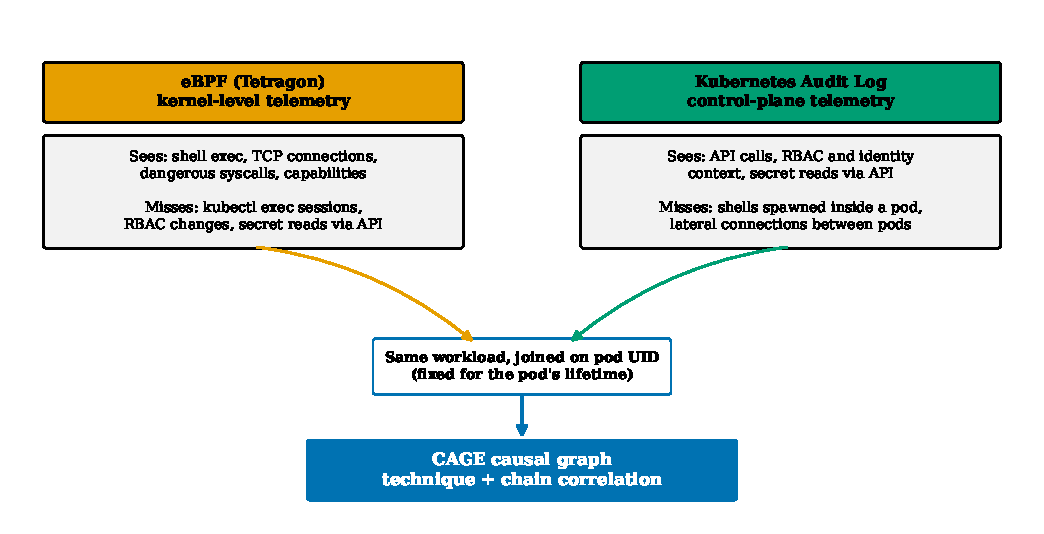
\includegraphics[width=0.88\columnwidth]{fig1_visibility_gap.pdf}
\caption{The cross-layer visibility gap. eBPF and the Kubernetes audit
log each see roughly half of an attacker's actions inside a cluster;
CAGE joins the two streams on the pod UID, the one identifier that is
stable across both.}
\label{fig:visibility-gap}
\end{figure}

Kernel-level telemetry, gathered through eBPF \cite{ref17}, sees what a
process actually does once it is running inside a container: a shell being
spawned, a TCP connection being opened, a dangerous syscall being
invoked. It has no native concept of a Kubernetes API action, so a
\texttt{kubectl exec} session or a secret read through the API server produces
nothing for it to observe. Falco \cite{ref1} and Cilium Tetragon \cite{ref2}, the two
most widely deployed open-source runtime security tools for Kubernetes,
both work this way. They instrument the kernel through eBPF or a
kernel-module probe and evaluate each syscall- or process-level event
against a rule set, independently of anything happening at the control
plane.

Control-plane telemetry, the Kubernetes audit log, sees the opposite
half of the picture. It records every API action along with full
identity and RBAC context, but it is blind to what happens once a
connection or session is actually established inside a container; it
cannot see a shell being spawned, nor a lateral connection opened
between two pods. K8NTEXT \cite{ref3} works from this side of the boundary,
reconstructing the causal structure that the audit log otherwise
scatters across thousands of loosely related entries, but its telemetry
remains the audit log and nothing else. Each of these tools is mature
and effective within its own telemetry source. None of them looks at
the other source at all, and none was designed to.

The cost of this single-source design is not just unseen events; it is
that many events either tool does see are individually ambiguous. A
routine \texttt{kubectl exec} to check a pod's health is indistinguishable,
from the audit log alone, from an attacker establishing a
remote-execution foothold, and an ordinary debugging shell looks, from
eBPF alone, exactly like a post-exploitation shell. What separates the
two is the sequence: a remote exec, followed by a shell, followed by a
secret read from inside that shell, all attributed to the same
workload, a materially stronger signal than any individual event. A
tool instrumenting only one side of the kernel/control-plane boundary
never observes that sequence, no matter how carefully tuned, and even
if it could see across the boundary, it has no source-independent
workload identity with which to link the observations together.

This gap has not been closed by prior work, although several projects
sit close to it. Falco and Tetragon operate exclusively on eBPF
telemetry, scoring each event independently with no mechanism to tie a
kernel-side event to a control-plane one. K8NTEXT operates exclusively
on the audit log: it reconstructs which control-plane events a given
action caused, but cannot see what happened inside the pod as a
result, so it misses the shell a correlated \texttt{kubectl exec} spawns. PACED
\cite{ref4}, UNICORN \cite{ref5}, and P4Control \cite{ref8} form a broader family of
provenance- and information-flow-based systems CAGE is architecturally
closer to, but each targets a narrower problem: PACED detects only
container escape via kernel provenance, UNICORN is a general,
non-Kubernetes anomaly detector for slow APT campaigns rather than
technique-level classification, and P4Control enforces
information-flow policy at the network layer, a prevention mechanism
rather than the after-the-fact detection and chain correlation this
paper addresses. No existing system fuses eBPF telemetry with the
Kubernetes audit log through a stable, workload-level identity key to
detect and correlate a broad MITRE ATT\&CK technique catalog.

CAGE closes this gap using the Kubernetes pod UID as an explicit
correlation key across both telemetry sources. Unlike a pod's name or
IP address, the UID is assigned once by the Kubernetes API server and
stays fixed for the pod's entire lifetime, so it can be resolved
through the watch API, cached, and used to tie an eBPF-sourced event and
an audit-log-sourced event back to the same workload without guessing.
Events from either source that share a pod UID are linked into a single
causal graph, and sequences of technique detections that match one of
five documented multi-hop attack patterns are escalated into a CRITICAL
correlated-chain alert, which carries stronger evidentiary weight than
any single per-technique alert on its own.

We evaluate CAGE along two axes, each organized around explicit
research questions and answered entirely through live-cluster trials
rather than simulation. These two axes are not independent concerns: a
detector that catches every attack but adds unpredictable latency,
consumes unbounded resources, or fails silently when part of the
infrastructure goes down is not something an operator could actually
run in production, so we treat detection quality and systems
characteristics as two halves of a single evaluation rather than as
separate studies.

\emph{Detection quality:}
\begin{itemize}
\item \textbf{RQ1.} How accurately does CAGE detect each of its eleven
  techniques individually, and does that accuracy hold consistently
  across techniques with a deliberate scope exclusion as well as those
  without one? (\S\ref{subsec:rq1})
\item \textbf{RQ2.} Is full detection coverage achievable from either telemetry
  source alone, or does covering the entire technique catalog
  structurally require fusing both? (\S\ref{subsec:rq2})
\item \textbf{RQ3.} Does CAGE's chain correlator detect independent instances of
  the same multi-step attack against the same workload reliably and
  repeatedly, confirming that its episode-scoped deduplication design
  works as intended? (\S\ref{subsec:rq3})
\item \textbf{RQ4.} For CAGE's threshold-based detectors, exactly where does the
  line between evasion and detection fall relative to the documented
  default thresholds? (\S\ref{subsec:rq4})
\end{itemize}

\emph{Systems characteristics:}
\begin{itemize}
\item \textbf{RQ5.} What is CAGE's end-to-end detection latency, and does that
  latency depend systematically on which telemetry source produced the
  underlying event? (\S\ref{subsec:rq5})
\item \textbf{RQ6.} How much CPU and memory overhead does CAGE add to its host,
  both at idle and under active attack load? (\S\ref{subsec:rq6})
\item \textbf{RQ7.} Does CAGE's pod-to-pod network-monitoring subsystem continue
  to perform consistently as the number of monitored pods grows? (\S\ref{subsec:rq7})
\item \textbf{RQ8.} Can CAGE recover its functionality after realistic
  infrastructure faults without an operator having to intervene?
  (\S\ref{subsec:rq8})
\end{itemize}

\textbf{Contributions.} The contributions of this paper are summarized as
follows:

\begin{itemize}
\item We present CAGE, a cross-layer runtime security architecture that
  fuses eBPF process and network telemetry with Kubernetes audit-log
  events through a live, watch-API-backed pod-identity cache. CAGE
  detects 11 MITRE ATT\&CK techniques and correlates them into five
  documented multi-hop attack chains with episode-scoped deduplication
  (\S\ref{sec:threat-model}--\S\ref{sec:system-design}).
\item We evaluate CAGE's detection quality on live infrastructure against
  four explicit research questions, reporting per-technique accuracy
  backed by Wilson confidence intervals, a telemetry-source ablation
  study, chain-correlation reliability across independent episodes, and
  an evasion-boundary characterization of the system's threshold-based
  detectors (\S\ref{subsec:rq1} through \S\ref{subsec:rq3} and \S\ref{subsec:rq4}).
\item We evaluate CAGE's systems characteristics on the same live
  infrastructure, reporting detection latency, resource overhead,
  monitoring-subsystem scalability, and functional recovery from
  injected infrastructure faults, each with appropriate confidence
  intervals rather than bare point estimates (\S\ref{subsec:rq5} through \S\ref{subsec:rq7} and \S\ref{subsec:rq8}).
\item We report two systems findings that revise or confirm specific design
  decisions rather than simply characterizing performance: a highly
  consistent 27.96-second Tetragon-sourced detection-latency plateau
  whose relationship to connection age we report honestly as an open
  question (\S\ref{subsec:rq5}), and direct evidence that a concurrent-polling fix to
  the pod-to-pod network monitor keeps cycle time flat across the tested
  scale range, correcting an earlier design that could split a single
  scan-burst attack across two polling cycles and let it evade detection
  entirely (\S\ref{subsec:rq7}).
\item We report and analyze a set of real detection-logic and
  evaluation-tooling defects, found independently across both halves of
  this evaluation effort, that surfaced only once each experiment ran
  against live infrastructure rather than under code review or
  synthetic testing. We argue this generalizes into a methodological
  point: systems whose correctness depends on multi-source event timing
  and cross-process state need to be evaluated against live
  infrastructure, not only reasoned about on paper (\S\ref{sec:lessons}).
\end{itemize}

The rest of this paper is organized as follows. Section~\ref{sec:related-work} surveys
related work. Section~\ref{sec:threat-model} states the threat model. Section~\ref{sec:system-design} describes
CAGE's architecture. Section~\ref{sec:eval-methodology} details the evaluation methodology.
Section~\ref{sec:results} presents results for each research question. Section~\ref{sec:lessons}
discusses lessons learned from building the evaluation infrastructure
itself. Section~\ref{sec:limitations} states limitations and threats to validity.
Section~\ref{sec:conclusion} concludes.

\section{Related Work}
\label{sec:related-work}

MITRE ATT\&CK \cite{ref9} is the common vocabulary this paper builds on: a
curated, publicly maintained catalog of adversary tactics and
techniques, originally scoped to enterprise IT and since extended to
cloud and containerized environments. A recent systematization of the
research literature found ATT\&CK used across cyber threat intelligence,
intrusion detection, red-team exercises, and risk assessment, spanning
enterprise networks, industrial control systems, and mobile platforms
\cite{ref10}. CAGE maps each of its eleven detected behaviors to a base ATT\&CK
technique identifier, in one case (T1548-PRIV-POD) extended with a
project-defined suffix naming a specific privileged-pod-creation
variant rather than a published sub-technique, so its coverage claims
can be compared directly against the
ATT\&CK-mapped systems discussed below.

\subsection{Kernel-Level Runtime Security via eBPF}
\label{subsec:rw-ebpf}

Falco \cite{ref1}, originally developed by Sysdig and now CNCF-graduated,
monitors kernel syscalls via eBPF or a kernel-module probe against a
customizable rule set, enriching events with container and Kubernetes
metadata before forwarding alerts downstream. Cilium Tetragon \cite{ref2}
similarly instruments process execution and network events through
eBPF \texttt{TracingPolicy} objects. eBPF-PATROL \cite{ref11} intercepts syscalls and
execution context to enforce user-defined policies against reverse
shells, privilege escalation, and container escape, with reported
overhead under 2.5\%. All three operate purely at the kernel boundary:
none ingests the Kubernetes audit log or relates a syscall-visible
event to the API-level action that may have caused it. CAGE uses
Tetragon as its eBPF producer but adds the audit-log and correlation
layers none of these tools provide.

\subsection{Audit-Log-Based Detection}
\label{subsec:rw-audit}

K8NTEXT \cite{ref3} (Franzil et al., \emph{Computer Networks}, 2026) addresses a
related but different problem: Kubernetes audit logs record each API
call largely independently, so the secondary events a single user
action triggers are scattered through the log with little explicit
linkage. K8NTEXT reconstructs \emph{contexts}, groupings of an actor's action
with the downstream events it caused, using inference rules plus a
deep-learning model, reporting over 95\% grouping accuracy on
operations involving up to 100+ correlated entries. This is a
log-\emph{structuring} system, scoped to the audit log alone; it cannot
observe the kernel-side half of a chain such as T1021$\to$T1059 (remote
exec, visible in the audit log, followed by the shell it spawns,
visible only via eBPF).

\subsection{Provenance and Information-Flow-Based Systems}
\label{subsec:rw-provenance}

PACED \cite{ref4} (Abbas et al., IC2E 2022) targets a narrower, high-severity
problem, container \emph{escape}, defining what constitutes a cross-namespace
event and proposing a \texttt{privileged\_flow} rule evaluated against a
benchmark of real container-escape CVEs with near-perfect accuracy and
no false negatives. UNICORN \cite{ref5} (Han et al., NDSS 2020) is a general,
non-Kubernetes host-level anomaly detector that incrementally sketches
whole-system provenance graphs to catch long-running, low-and-slow APT
campaigns without predefined signatures. KAIROS \cite{ref12} (Cheng et al.,
IEEE S\&P 2024) extends this line of work with a graph-neural-network
encoder-decoder that learns how a provenance graph evolves over time,
detecting cross-application attacks without prior signatures while
reconstructing a human-readable summary; PACED, UNICORN, and KAIROS
share a co-author (Thomas Pasquier) and form one continuous research
thread CAGE sits adjacent to rather than inside. P4Control \cite{ref8}
(Bajaber et al., IEEE S\&P 2024) instead enforces decentralized
information-flow-control policy at line rate using programmable (P4)
network switches plus a lightweight host-side eBPF primitive, a
prevention mechanism rather than a detection one. None of these four
systems is Kubernetes-specific or performs technique-level MITRE
ATT\&CK mapping across a broad catalog; CAGE's contribution here is
orthogonal to theirs rather than a direct improvement on any one.

\subsection{Multi-Stage Attack and Alert Correlation}
\label{subsec:rw-correlation}

A separate line of work addresses the analyst-facing side of
multi-stage attacks: the sheer alert volume a real deployment
generates. Wilkens et al. \cite{ref13} synthesize kill chain state machines
from network alert streams, condensing up to 446,458 raw alerts from
the CSE-CIC-IDS2018 dataset into roughly 700 human-reviewable attack
scenario graphs, using network topology and zone directionality to
infer plausible attack-stage transitions, over general enterprise
network alerts rather than Kubernetes-specific events, discovering
open-ended scenario graphs rather than matching a fixed catalog. CAGE's
chain correlator addresses a structurally similar problem, reducing
per-technique alerts to a small number of high-confidence chain
alerts, but keys correlation to a Kubernetes pod UID and evaluates
against five specific, pre-documented ATT\&CK chains rather than
deriving arbitrary scenario
graphs from network-layer alerts alone.

\subsection{Positioning of CAGE}
\label{subsec:rw-positioning}

Table~\ref{tab:related-work} summarizes this comparison along five axes: telemetry
sources, multi-hop chain detection, Kubernetes pod-identity
correlation, live attack-graph visualization, and false-positive
mitigation strategy. Falco and vanilla Tetragon are included alongside
the systems discussed above because they are the two most directly
comparable deployed tools: Falco as the dominant open-source
Kubernetes runtime-security tool, and vanilla Tetragon as the
single-source baseline CAGE itself is built on and extends.

\begin{table*}[!t]
\centering
\caption{Related-Work Feature Comparison.}
\label{tab:related-work}
\setlength{\tabcolsep}{3pt}
\tablebodyfont
\renewcommand{\arraystretch}{1.05}
\begin{tabular}{@{}>{\raggedright\arraybackslash}p{0.070\textwidth}>{\raggedright\arraybackslash}p{0.150\textwidth}>{\raggedright\arraybackslash}p{0.180\textwidth}>{\raggedright\arraybackslash}p{0.180\textwidth}>{\raggedright\arraybackslash}p{0.160\textwidth}>{\raggedright\arraybackslash}p{0.180\textwidth}@{}}
\toprule
\textbf{System} & \textbf{Telemetry Sources} & \textbf{Multi-Hop Chain Detection} & \textbf{Kubernetes Pod-Identity Correlation} & \textbf{Live Attack-Graph Dashboard} & \textbf{False-Positive Mitigation} \\
\midrule
K8NTEXT & Kubernetes audit log only & Context-grouping across correlated actions, not MITRE-technique-level chain detection & Not specified in the published evaluation & Not applicable & Inference rules plus a machine-learning grouping model (over 95\% accuracy) \\
UNICORN & Host-level provenance graph, source-agnostic; not confirmed eBPF-based & Anomaly-based long-range correlation, not Kubernetes-specific, not technique-level & Not applicable; not Kubernetes-scoped & Not applicable & Provenance-graph anomaly scoring \\
PACED & Kernel provenance capture & Single-hop; container-escape events only & Not specified & Not applicable & \texttt{privileged\_flow} rule evaluated against a CVE benchmark \\
KAIROS & Host-level provenance graph via graph neural network & Anomaly-based, cross-application scope; not Kubernetes-specific, not technique-level & Not applicable; not Kubernetes-scoped & Not applicable & Learned graph-embedding anomaly scoring \\
P4Control & Programmable (P4) network switches plus lightweight host eBPF & Single-hop; in-network information-flow-control label propagation & Not applicable; not Kubernetes-scoped & Not applicable & DIFC label-based line-rate enforcement \\
Falco & eBPF or kernel-module syscall monitoring & None; single-event rules & Partial (Kubernetes metadata enrichment on syscall events, not a correlation key) & Not built in (a separate, optional UI component exists) & Static rule tuning; no built-in behavioral-burst thresholds \\
Vanilla Tetragon & eBPF only (process exec, network, file, capabilities) & None; per-policy alerts with no cross-event correlation & Native Kubernetes metadata on events, but not used as an explicit cross-source join key & Hubble UI, network-flow visualization; not an attack-chain view & Per-policy filtering only \\
\textbf{CAGE} & \textbf{eBPF (Tetragon) plus Kubernetes audit log plus pod-UID watch} & \textbf{Multi-hop; five documented chain types} & \textbf{Pod UID as an explicit correlation key across all sources} & \textbf{Yes: attack-graph canvas, kill-chain stepper, MITRE matrix, per-source health status} & \textbf{Namespace-scope exclusion, scan-burst thresholds for T1610, remote-exec correlation windows for T1059} \\
\bottomrule
\end{tabular}
\end{table*}

This is explicitly a qualitative comparison against each system's own
published description, not a quantitative benchmark; no other tool was
run against CAGE's own attack set in this project's cluster.
\S\ref{sec:conclusion} identifies a concrete, low-effort path to a
direct quantitative comparison as future work.

\section{Threat Model}
\label{sec:threat-model}

\textbf{In scope.} An attacker who has already obtained code execution inside
one pod, whether through a vulnerable application, a supply-chain
compromise, or a misconfigured or leaked credential, and who then
attempts to escalate: spawning shells, moving laterally to other pods,
reading Kubernetes secrets, escalating privileges inside or outside the
container, abusing RBAC, or degrading node resources. This matches the
11 techniques in Table~\ref{tab:techniques}.

\textbf{Trust assumptions.} The Linux kernel and eBPF subsystem are trusted;
an attacker capable of loading rogue eBPF programs or otherwise blinding
Tetragon's hooks defeats the detection substrate itself, a limitation
shared by any eBPF-based defense and not specific to CAGE. The
Kubernetes API server and its audit log are trusted; an attacker with
control-plane-level access sufficient to disable or tamper with audit
logging is operating at a privilege level well beyond one compromised
workload pod. CAGE's own process is trusted and assumed uncompromised.
By design, CAGE performs only read operations against the Kubernetes
API, watching and listing pods for identity resolution and reading the
audit log stream, and it never creates, modifies, or deletes any
cluster resource, so compromising CAGE itself would grant no write
capability beyond what a compromised workload already has. In this
evaluation, however, CAGE authenticates with the same local kubeconfig
used to administer the cluster rather than a purpose-built,
minimally-scoped ServiceAccount, so its actual runtime credentials are
broader than its architecture requires; replacing this with a
dedicated read-only ServiceAccount is straightforward but had not been
done as of this evaluation. The fault-injection evaluation (\S\ref{subsec:rq8})
tests CAGE's resilience to \emph{infrastructure} failures affecting its own
components, a reliability property, not a defense against an adversary
who has already compromised CAGE itself.

\textbf{Explicitly out of scope.} Kernel- or eBPF-blinding rootkits, as
noted above; supply-chain-introduced malware whose runtime behavior
falls entirely outside the 11 watched techniques, for example pure
data exfiltration over an already-open, legitimate network connection
with no new shell, connection, or privileged action involved; single
events that are individually indistinguishable from legitimate
administrative activity when viewed in isolation, which is precisely
the motivating case for chain correlation (\S\ref{subsec:rq3}); and multi-cluster
lateral movement. The last of these is a deliberate scoping decision
rather than an oversight: Kubernetes only guarantees pod UID uniqueness
within a single cluster's control plane, so using it as a correlation
key across independently administered clusters would require folding a
cluster identifier into the key and watching multiple API servers
concurrently, neither of which this version of CAGE implements.

\textbf{Known, deliberately measured boundary.} Several detection rules use
fixed numeric thresholds: a 5-distinct-destination burst for T1610, a
25-execution burst for T1499, and a 10-read burst for T1613. An attacker
aware of these values and disciplined enough to remain under them evades
the specific rule tuned against them. Rather than leave this as an
implicit, undisclosed limitation, RQ4 and \S\ref{subsec:rq4} measure exactly where
that boundary sits.

\section{System Design}
\label{sec:system-design}

\subsection{Design Objectives and Architectural Overview}
\label{subsec:design-overview}

The design problem CAGE addresses is not simply that eBPF and the
Kubernetes audit log each see half of an attack; it is that fusing them
requires a join key, and neither surface identifier qualifies. Pod
name is reusable across restarts and, adversarially, chosen by
whoever creates the pod: an earlier version of this codebase excluded
its own infrastructure by matching a pod-name prefix, later recognized
as a real evasion path since any workload matching the pattern,
including an attacker's own pod, went unwatched. Pod IP is likewise
reused as pods churn and is not always resolvable at the instant an
event is produced, since Kubernetes propagates identity through a
watch stream updating on its own schedule, independent of eBPF's
kernel event stream. CAGE instead uses the pod UID: assigned once by
the Kubernetes API server, stable for the pod's lifetime, and not
influenceable by a workload or attacker. Every design decision in this
section follows from committing to that identifier as the single
correlation key across telemetry sources that otherwise share no
vocabulary.

CAGE runs as a single Python process with several daemon threads
communicating through one shared, in-process event queue. A pod UID
cache thread maintains a live view of cluster identity by watching the
Kubernetes API. Two consumer threads, one for Tetragon's eBPF event
stream and one for the Kubernetes audit log, independently tag every
event they observe with a pod UID before placing it on the shared queue.
A third, thread-pool-backed consumer polls pod network state directly as
a complementary source for lateral-movement detection. A single
correlator loop drains the shared queue and evaluates each event against
a bounded per-identity temporal window to decide whether a technique or
a multi-hop chain has fired. It then forwards both raw events and any
resulting alerts to a Flask server, which exposes a REST API and two
Server-Sent Events streams to a browser dashboard (Fig.~\ref{fig:architecture}).

\begin{figure}[!t]
\centering
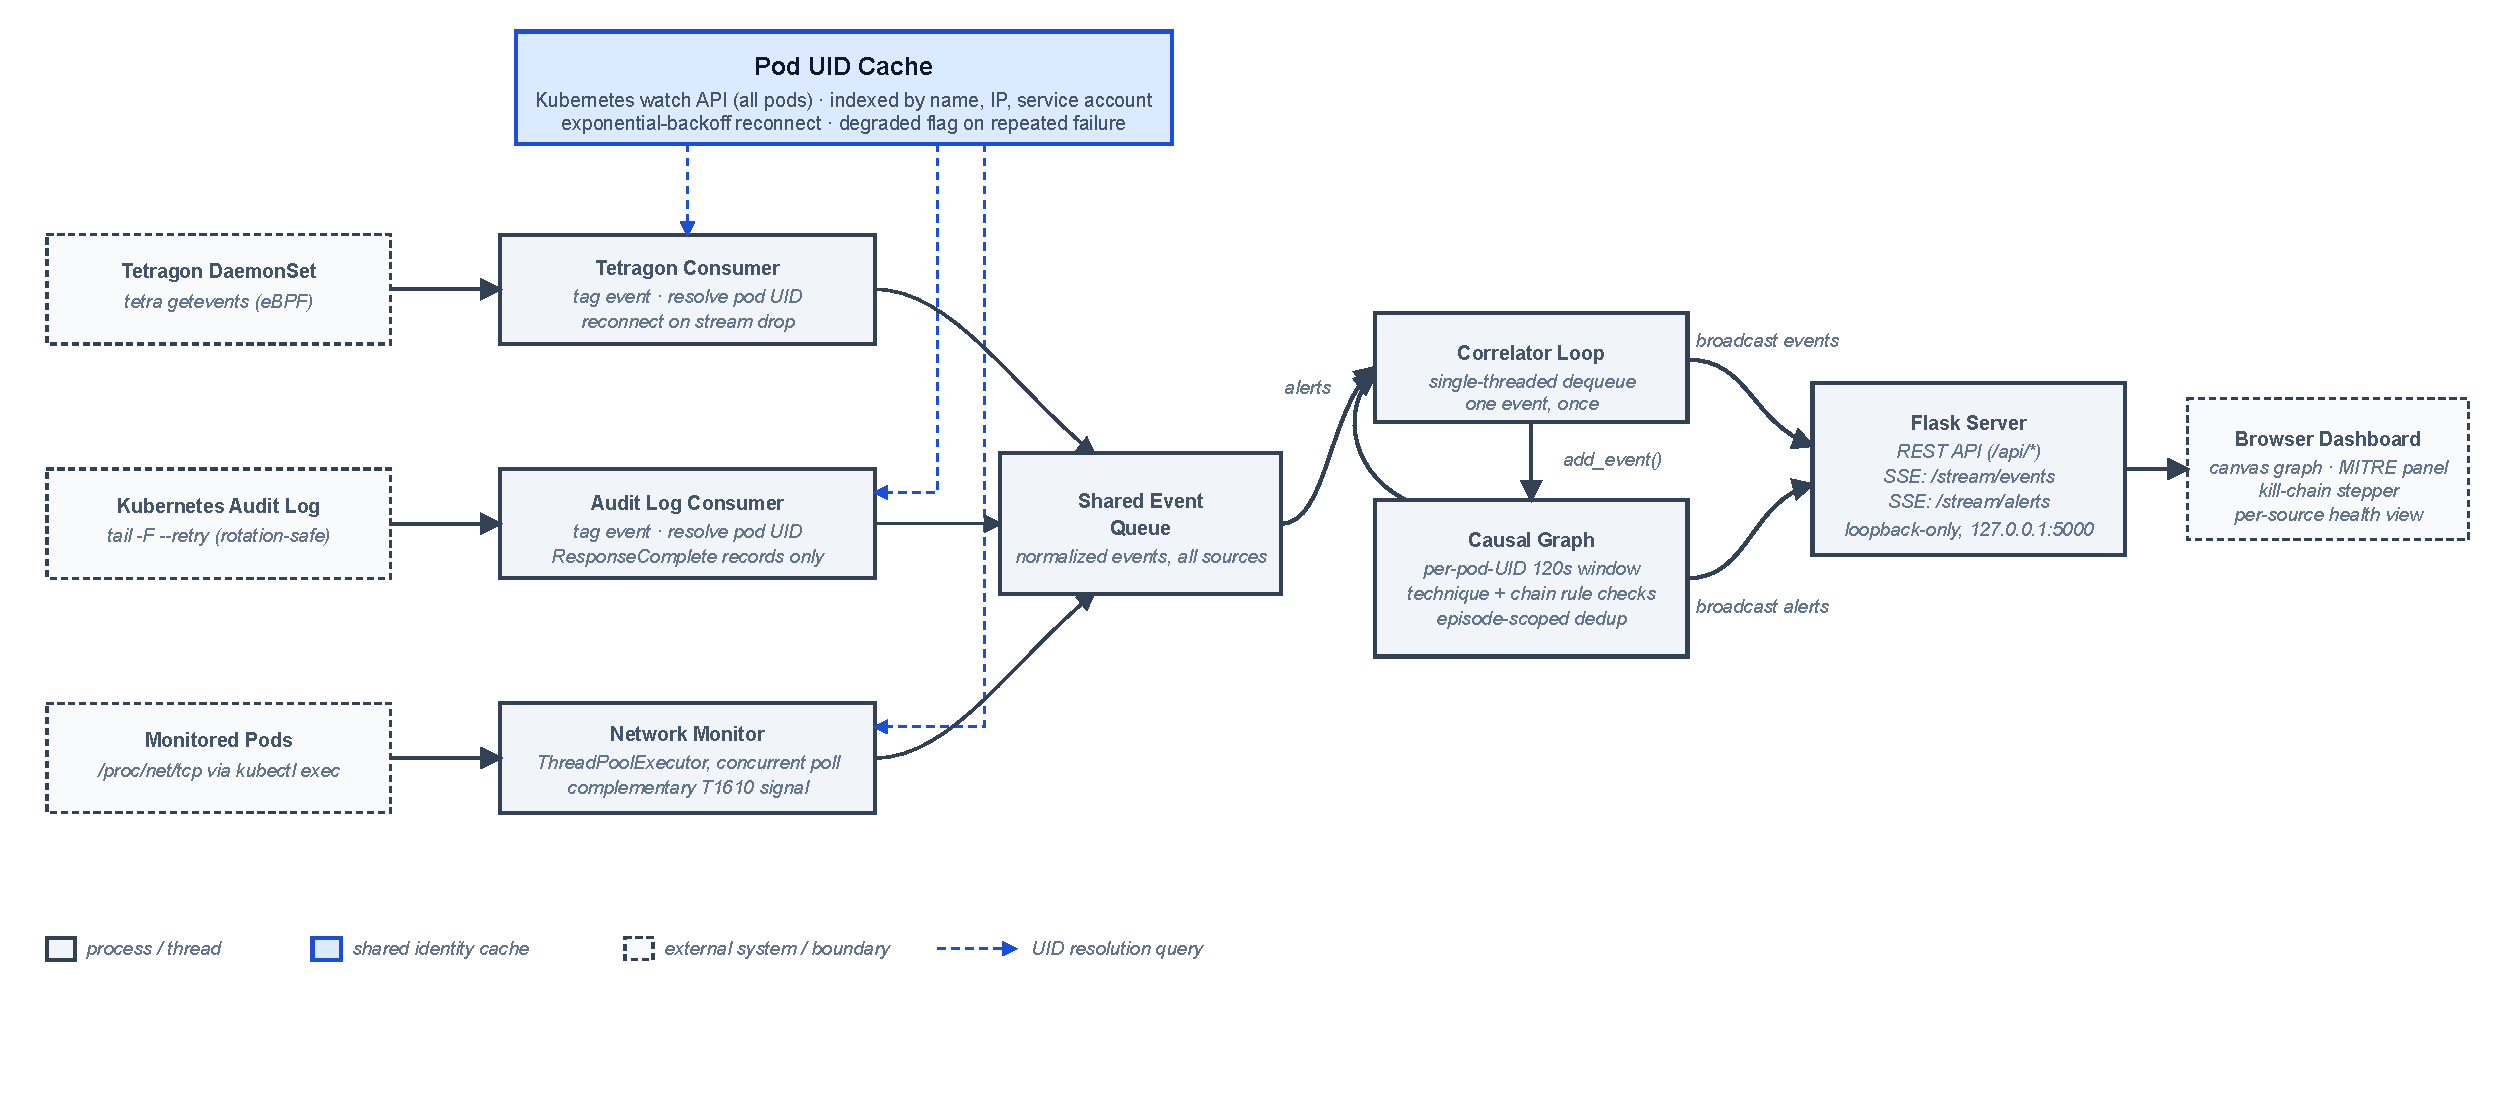
\includegraphics[width=\columnwidth]{fig2_architecture.pdf}
\caption{Overall CAGE architecture. The Tetragon consumer, audit-log
consumer, and network monitor each resolve pod identity against the
shared pod UID cache and tag every event before placing it on one
shared queue. A single correlator loop drains that queue, checks each
event against the causal graph's per-pod-UID window, and broadcasts
both raw events and resulting alerts through the Flask server to the
browser dashboard.}
\label{fig:architecture}
\end{figure}

Two consequences follow from this structure. First, the hardest
problem is not any individual detection rule but establishing pod
identity reliably and fast enough for two telemetry domains that learn
about it at different speeds; \S\ref{subsec:uid-resolution} describes
that mechanism, where most of this codebase's engineering effort went.
Second, once identity resolution and event normalization are handled,
the detection logic itself is deliberately simple: bounded state,
explicit thresholds, and no learned model between an event and an
alert, a trade-off \S\ref{subsec:temporal-correlation} explains
directly.

\subsection{Telemetry Acquisition}
\label{subsec:telemetry-acquisition}

CAGE draws on two structurally different telemetry domains and adds a
third, complementary signal for one specific technique.

The Tetragon consumer runs \texttt{tetra getevents} against Tetragon's DaemonSet
through a persistent \texttt{kubectl exec} subprocess, reading its JSON event
stream line by line. Two custom \texttt{TracingPolicy} resources extend
Tetragon's default process-execution visibility: one attaches a kprobe
to \texttt{tcp\_connect} to observe outbound connections at the socket layer,
and the other attaches a kprobe to \texttt{cap\_capable}, filtered to four
capability values (\texttt{CAP\_SYS\_ADMIN}, \texttt{CAP\_SYS\_PTRACE}, \texttt{CAP\_SYS\_MODULE},
\texttt{CAP\_SYS\_BOOT}) that indicate privilege escalation or container escape
rather than ordinary operation. If the subprocess exits or the stream
ends, the consumer reconnects after a short fixed delay rather than
escalating to a supervisor-level restart, since a missed handful of
seconds of kernel telemetry is recoverable in a way a crashed process
is not.

The audit log consumer tails the API server's audit log file inside
the control-plane container using \texttt{tail -F --retry} rather than the more
common \texttt{-f}, since Kubernetes rotates the log in place once it reaches
a configured size: \texttt{-f} follows a file descriptor that rotation
invalidates, silently orphaning the reader, while \texttt{-F} reopens the path
by name and survives it. The consumer only acts on records whose
\texttt{stage} is \texttt{ResponseComplete}; earlier stages describe a request not yet
authorized or completed, and treating one as alert-worthy would let a
denied request masquerade as a successful one.

A third source, the network monitor, addresses a limitation of relying
on the \texttt{tcp\_connect} kprobe alone for lateral-movement detection: kprobe
coverage depends on a BTF-enabled kernel, a constraint
(\S\ref{sec:limitations}) that does not hold across every deployment.
The network monitor is an independent, poll-based fallback that
periodically executes \texttt{cat /proc/net/tcp} inside every monitored pod
through \texttt{kubectl exec} and parses established connections directly from
procfs, requiring no kernel-level instrumentation, which makes it a
genuinely complementary signal for the same technique (T1610) rather
than a duplicate of the kprobe path. Because polling is not free,
monitoring every pod sequentially made sweep time grow with pod count;
once that time exceeded the detection rule's own burst window, a
genuine multi-destination scan could split across two sweeps and never
accumulate enough distinct destinations in one window to cross the
threshold, a defect surfaced during development rather than
anticipated up front. The fix polls all monitored pods concurrently
through a thread pool sized to the pod count, bounding sweep time by
the slowest single \texttt{kubectl exec} call rather than their sum;
\S\ref{subsec:rq7} reports on this design's scalability directly.

\subsection{Pod UID Identity Resolution}
\label{subsec:uid-resolution}

Resolving a pod UID from the audit log is comparatively direct: certain
record types, in particular a Secret access performed from inside a
pod using its mounted service account token, carry pod name and UID as
structured fields under the request's \texttt{user.extra} metadata, placed
there by the API server itself rather than inferred by CAGE. Resolving
a pod UID from an eBPF event is not direct at all, and this is where
the identity race described in \S\ref{subsec:design-overview} actually
has to be handled.

The pod UID cache is populated by a long-running Kubernetes watch over
all pods across all namespaces, thread-safe and indexed three ways: by
\texttt{(namespace, name)}, by pod IP, and by \texttt{(namespace, service account)}.
The watch reconnects with exponential backoff on failure; once
failures cross a small consecutive-failure threshold, the cache
exposes a \texttt{degraded} flag distinguishing ``no recent activity'' from
``identity resolution is not currently trustworthy.'' This flag is
informational and does not gate detection, a separation of concerns
\S\ref{subsec:alert-dashboard} discusses further.

Tetragon events do not always carry a usable pod reference directly.
When they do, resolution is immediate via the event's own \texttt{pod.uid}
field; when they do not, and Tetragon reports only a raw container
identifier, CAGE falls back to a container-ID map built once at
startup and refreshed every three seconds from the Kubernetes API's
own container status records, matched against Tetragon's own prefix
lengths for that identifier. The three-second cadence balances two
costs: refreshing per event would query the API once per exec, which
does not scale with event volume, while a much longer interval would
leave short-lived containers unresolvable for most of their existence.
The consumer also learns container-ID associations directly from
\texttt{runc} invocations in the same event stream, extracting the identifier
from the invocation's arguments and caching it immediately rather than
waiting for the next periodic refresh.

Even with both mechanisms running, a process can execute and be
reported by eBPF before either resolves its container. Rather than
dropping these events silently or blocking the consumer thread, CAGE
places any plausibly container-referencing event in a small retry
buffer, re-attempted every 300 milliseconds for up to two seconds;
anything still unresolved after that window is dropped and logged
explicitly, since an event un-attributable after two seconds is
unlikely to become attributable later (Fig.~\ref{fig:uid-resolution}).

\begin{figure}[!t]
\centering
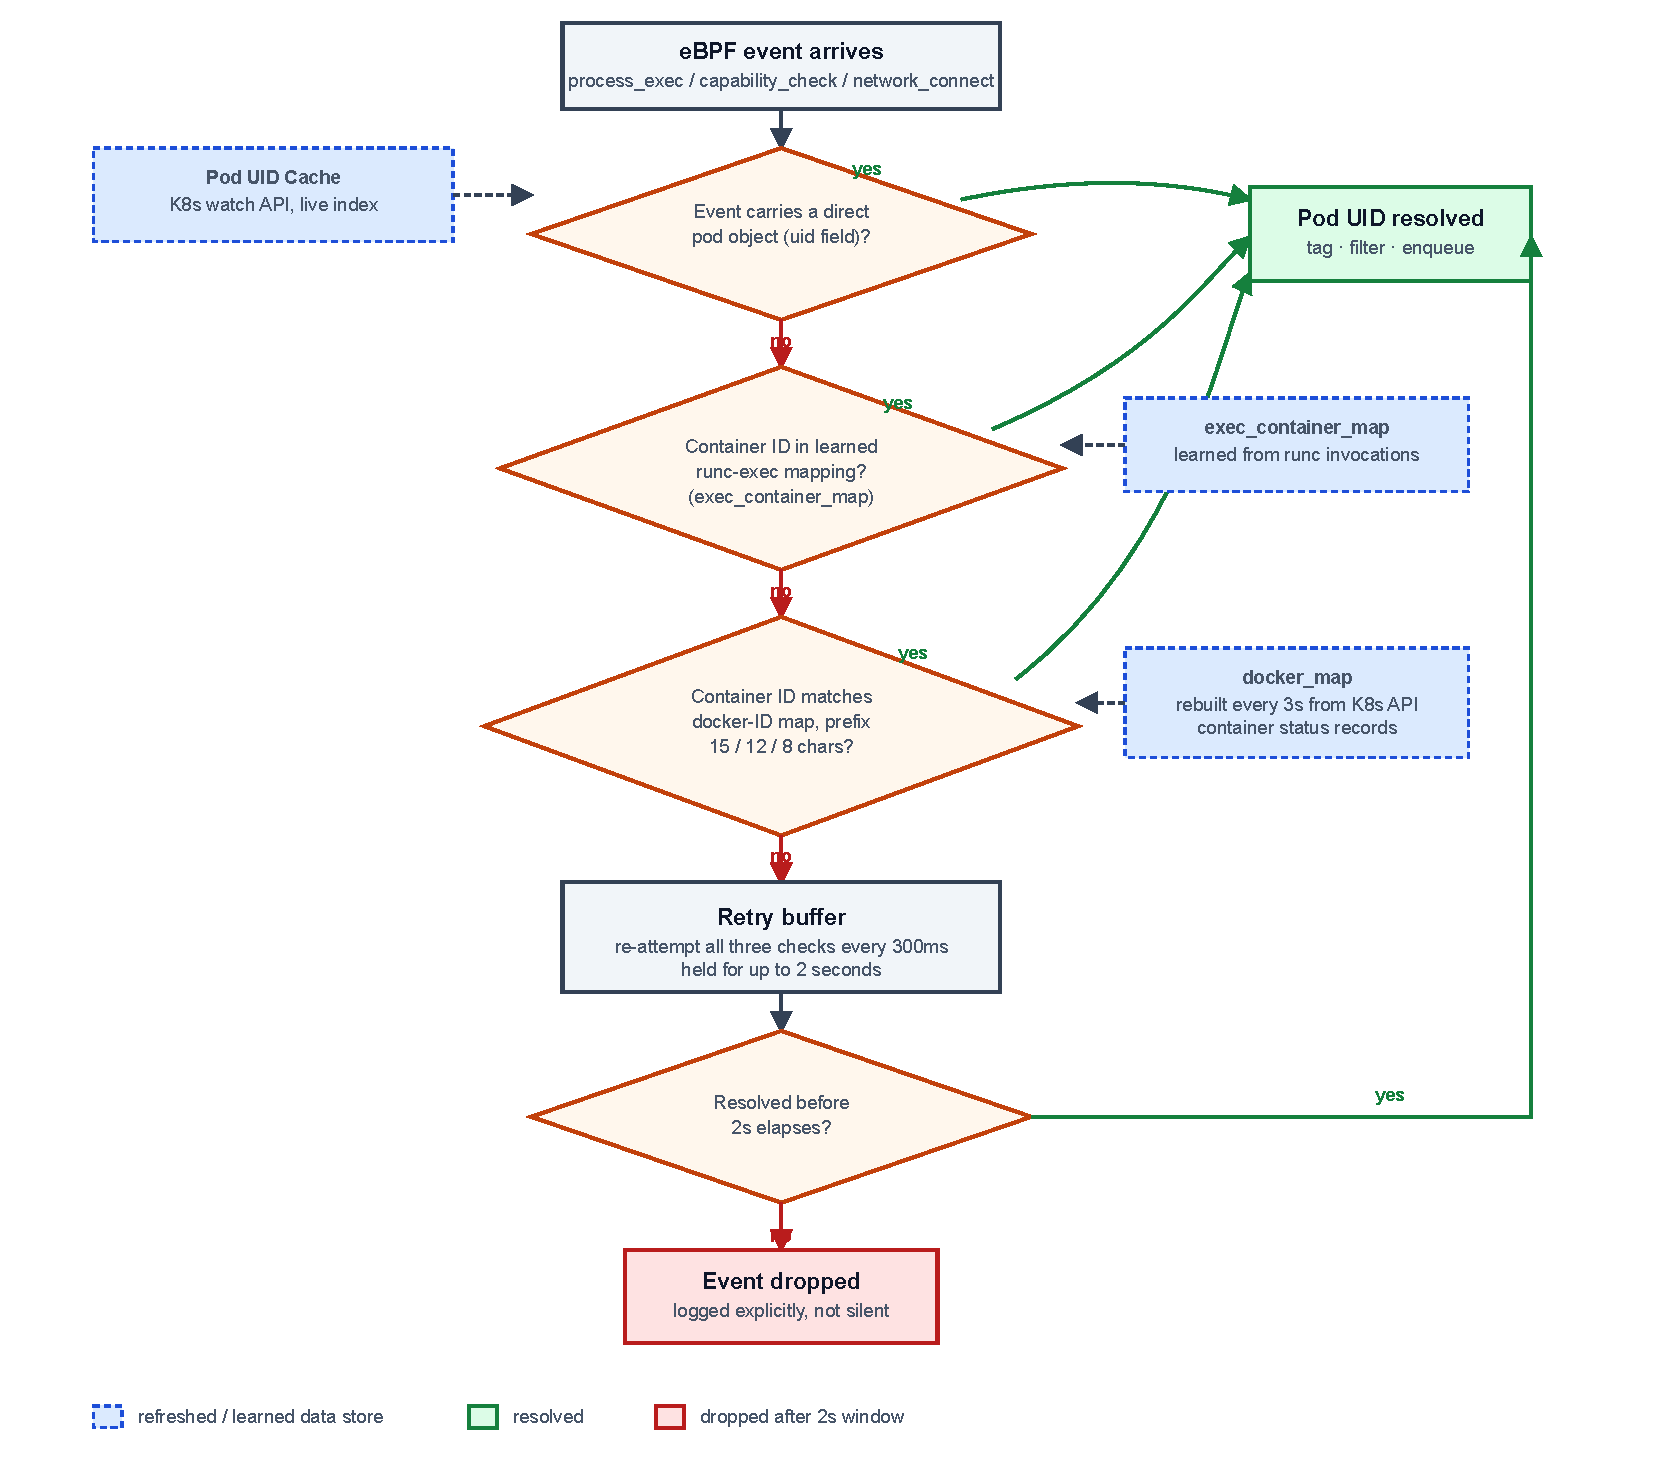
\includegraphics[width=0.75\columnwidth]{fig3_uid_resolution.pdf}
\caption{Pod UID resolution workflow for an incoming eBPF event. A
direct pod object resolves immediately; otherwise the consumer checks
its container-ID map learned from \texttt{runc} invocations, then the map
rebuilt every three seconds from the Kubernetes API, before falling
back to the retry buffer, which re-attempts all three checks every 300
milliseconds for up to two seconds before dropping the event.}
\label{fig:uid-resolution}
\end{figure}

Every event tagging function additionally discards events whose
resolved namespace falls in a small set of cluster-infrastructure
namespaces before the event is queued at all, rather than only inside
each detection rule, a distinction that matters beyond correctness: a
live measurement on an otherwise idle cluster found cluster-infrastructure
activity, chiefly \texttt{kube-proxy}'s continual iptables resynchronization,
accounted for 77\% of total eBPF event volume, and letting all of it
reach the queue only to be discarded downstream would waste processing
time on events that can never produce an alert either way.

\subsection{Event Normalization}
\label{subsec:event-normalization}

Tetragon and the audit log describe events in vocabularies that share
almost nothing. A Tetragon process-execution event is a kernel-level
record of a binary, its arguments, and its process lineage; an audit
record is a control-plane request described by verb, resource type, and
requesting identity. CAGE's normalization layer, implemented separately
in each consumer, converts both into one common event shape before
either is exposed to a detection rule. {\sloppy That shape has an \texttt{event\allowbreak\_type}
field (\texttt{process\allowbreak\_exec}, \texttt{capability\allowbreak\_check}, \texttt{network\allowbreak\_connect},
\texttt{k8s\allowbreak\_secret\allowbreak\_access}, \texttt{pod\allowbreak\_exec}, \texttt{privileged\allowbreak\_pod\allowbreak\_created}, \texttt{rbac\allowbreak\_abuse},
\texttt{rbac\allowbreak\_discovery}), a resolved pod UID, pod name, and namespace, a
timestamp, and a small number of fields specific to that event type.} This
common shape is what makes the rest of the system source-agnostic. The
correlation logic that follows operates entirely on this normalized
representation and has no notion of which telemetry domain an event
originated from, except for the source attribution kept for
observability.

\subsection{Temporal Correlation and the Causal Graph}
\label{subsec:temporal-correlation}

The correlation engine is deliberately simpler than its name suggests.
\texttt{CausalGraph} maintains a \texttt{networkx} directed graph whose nodes are pod
identities, added as events arrive, but does not currently populate
edges; the graph the dashboard renders is synthesized independently
(\S\ref{subsec:alert-dashboard}). What actually decides whether a
technique or multi-hop chain has fired is a bounded, per-pod-UID
sliding window of recent normalized events, held for 120 seconds and
pruned against each new event's timestamp. Individual technique rules
test this window, or the incoming event alone, against explicit
conditions: a shell binary observed inside a pod, a burst of
connections to five or more distinct destination pods within ten
seconds, twenty-five or more process executions from one pod within
ten seconds, ten or more reads of RBAC objects by one identity within
thirty seconds; the remaining techniques in Table~\ref{tab:techniques}
follow the same pattern. Chain detection reuses the same window rather
than running a separate pass: a chain such as
remote-exec-then-shell-then-secret-access is checked by testing
whether the relevant event types or binaries co-occur within the same
120-second window for the same pod UID, not by traversing a persisted
graph structure.

This design is a deliberate trade-off: a learned, graph-based approach,
of the kind KAIROS \cite{ref12} and UNICORN \cite{ref5} take at the
operating-system level, can in principle generalize to attack patterns
nobody enumerated in advance, at the cost of a decision boundary that
depends on training data and is not fully disclosable. CAGE's
bounded-window approach cannot generalize beyond its explicit rule set,
but every alert it produces traces to one named rule and one disclosed
threshold, measured directly by the evasion-boundary evaluation in
\S\ref{subsec:rq4}, and keeps resource cost flat under load rather than
scaling with a model's inference cost, as reported in \S\ref{subsec:rq6}.

A pod UID is a long-lived identifier reusable across many separate,
unrelated incidents over a pod's lifetime; nothing in Kubernetes
destroys a pod merely because it triggered an alert, which has a
direct consequence for how chain state must be managed. A chain or
burst condition marked as fired permanently for that pod UID would
silently prevent any later, genuinely independent incident on the same
workload from ever being reported again, so CAGE's chain and burst
detectors are instead episode-scoped: a firing key is retained only
while its underlying condition remains continuously satisfied and is
discarded the moment it goes false, letting a later, separate episode
on the same identity fire the same rule again. An earlier version of
the fork-bomb detector (T1499) added its firing key once and never
removed it, so a pod that triggered it once could never trigger it
again; this defect was found during this project's own evaluation
effort and verified fixed live, by firing two independent bursts
against the same long-lived pod and confirming both were reported.
\S\ref{sec:lessons} discusses this and several related defects found the
same way, by running the system rather than only reading it.

The per-pod-UID state above accumulates for every pod that has ever
produced an event, and pods in a real deployment churn continuously,
so CAGE periodically sweeps and discards tracking state for any pod
UID with no activity in the last 120 seconds, the same duration as the
correlation window itself, on an event-count cadence rather than a
wall-clock timer, avoiding a dedicated background thread purely for
garbage collection.

\subsection{Attack Detection Pipeline and MITRE ATT\&CK Mapping}
\label{subsec:detection-pipeline}

Every normalized event, regardless of source, passes through the same
sequence: a fixed set of technique-specific checks, each independent of
the others, followed by the chain checks described above (Fig.~\ref{fig:detection-pipeline}).
Table~\ref{tab:techniques} lists the eleven MITRE ATT\&CK techniques CAGE currently maps
to a rule, the severity assigned to each, and the telemetry source
that produces it.

\begin{figure}[!t]
\centering
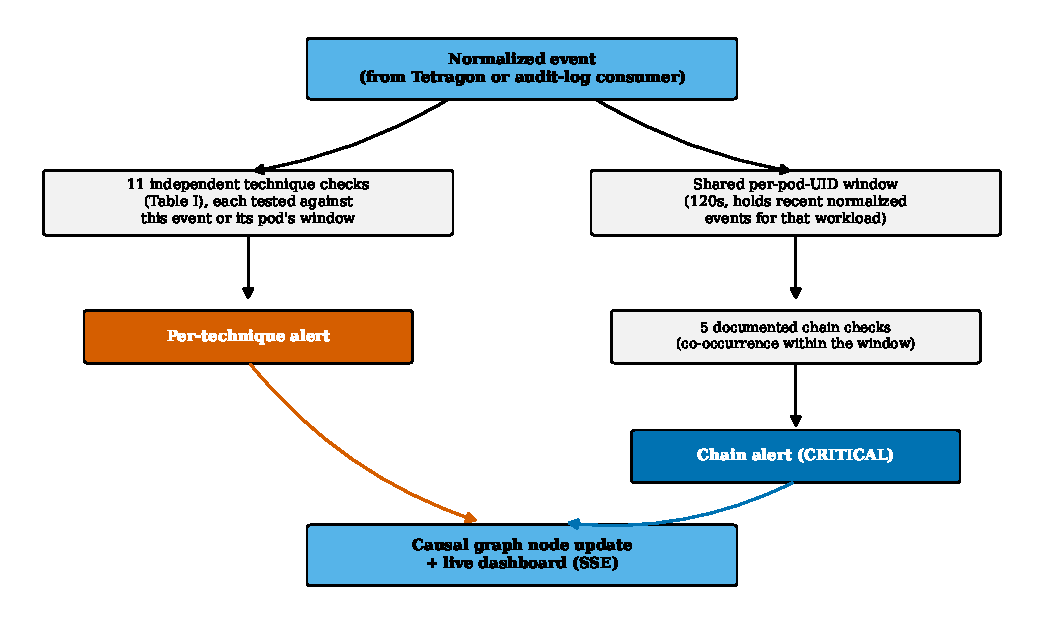
\includegraphics[width=0.9\columnwidth]{fig4_detection_pipeline.pdf}
\caption{The detection pipeline every normalized event passes
through. Technique checks run independently of one another; in
parallel, the shared per-pod-UID window feeds the five documented
chain checks. Both paths produce an output that updates the causal
graph and the live dashboard.}
\label{fig:detection-pipeline}
\end{figure}

\begin{table}[!t]
\centering
\caption{Detected MITRE ATT\&CK Techniques and Telemetry Source.}
\label{tab:techniques}
\tablebodyfont
\setlength{\tabcolsep}{2.5pt}
\begin{tabular}{@{}>{\raggedright\arraybackslash}p{0.23\columnwidth}>{\raggedright\arraybackslash}p{0.28\columnwidth}>{\raggedright\arraybackslash}p{0.14\columnwidth}>{\raggedright\arraybackslash}p{0.22\columnwidth}@{}}
\toprule
\textbf{Technique} & \textbf{Behavior} & \textbf{Severity} & \textbf{Source} \\
\midrule
T1059 & Shell spawned inside a pod & MEDIUM & Tetragon eBPF \\
T1021 & Remote exec (\texttt{kubectl exec}) & MEDIUM & K8s audit log \\
T1610 & Pod-to-pod network lateral movement (scan-burst) & MEDIUM & Tetragon kprobe + NetworkMonitor \\
T1552 & Secret access via K8s API & HIGH & K8s audit log \\
T1611 & Container escape (dangerous capability / escape binary) & HIGH & Tetragon eBPF \\
T1548 & Privilege escalation attempt inside a container & HIGH & Tetragon eBPF \\
T1548-PRIV-POD & Privileged pod created & HIGH & K8s audit log \\
T1548.005 & Cluster-admin / wildcard RBAC grant & CRITICAL & K8s audit log \\
T1496 & Cryptomining process signature & HIGH & Tetragon eBPF \\
T1499 & Fork-bomb-like exec burst (resource DoS) & HIGH & Tetragon eBPF \\
T1613 & RBAC / resource discovery burst & MEDIUM & K8s audit log \\
\bottomrule
\end{tabular}
\end{table}

Five multi-hop sequences of these techniques are escalated to a CRITICAL
correlated chain alert when their constituent legs are satisfied on the
same pod UID within the shared 120-second window. These are: T1059 to
T1552 (shell then credential access); T1021 to T1059 to T1552 (the full
remote-exec lateral-movement path); T1059 to T1610 to T1552 (shell, then
a network scan burst, then credential access); T1059 to T1548 to T1611
(shell, privilege escalation, then a container-escape indicator); and
T1611 to T1552 (an escape indicator followed by credential access). A
chain alert is strictly stronger evidence than any of its constituent
per-technique alerts on their own, since it requires several independent
detectors to agree on the same identity within a bounded time.

One rule is a deliberate, disclosed exception to an otherwise
consistent scope-exclusion policy: T1021 (\texttt{kubectl exec}) carries no
namespace exclusion at all, firing on any remote exec into any pod,
including routine administrative access into cluster-infrastructure
components. This precision cost is accepted deliberately, since
excluding infrastructure namespaces from this rule would also exclude
a real attacker's remote-exec session into a compromised
infrastructure pod, exactly the access it is meant to catch. Every
other behavioral rule excludes cluster-infrastructure namespaces
explicitly, by namespace rather than by pod name, for the same
evasion-resistance reason given in \S\ref{subsec:design-overview}.

\subsection{Alert Generation and Dashboard Integration}
\label{subsec:alert-dashboard}

Detection and visualization share the same event stream by
construction, not by two independent systems agreeing to stay in
sync: a single loop dequeues each normalized event once, evaluates it
against the causal graph, updates internal state, and pushes that
same event and any resulting alerts to two independent Server-Sent
Events subscriber sets, one for raw events and one for alerts, over a
REST API served by the same process. This matters for what the
dashboard can be trusted to show: the visualization layer consumes
exactly the events the detector consumed, so what an operator sees is
never a best-effort approximation of what was evaluated. The graph
itself, exposed through a \texttt{/api/graph} endpoint, is reconstructed on
each request directly from the current pod cache and accumulated
alert list rather than read back from a persisted structure inside
the correlator. Each pod node is colored by its highest observed alert
severity, and each alert type synthesizes its own edge: a self-loop
for an in-pod behavior such as a shell spawn or privilege escalation
attempt, a directed edge to a synthetic external node for a
remote-exec session, or an edge between two real pod nodes for a
lateral connection. The browser dashboard renders this as an
interactive canvas graph, alongside a MITRE technique reference panel,
a kill-chain \cite{ref18} step indicator for correlated alerts, and a
per-source health view.

That health view is deliberately kept separate from the detection
path. A \texttt{/api/health} endpoint reports, for each telemetry source,
whether its consumer is enabled, whether its subprocess is still
alive, and how long since it last produced an event, flagging a
source as stale once that silence passes a fixed threshold; none of
this bookkeeping influences whether an event is processed or an alert
fires. Its only purpose is making degraded telemetry health observable
rather than silently masked, a property the fault-injection evaluation
in \S\ref{subsec:rq8} exercises directly. The same separation applies to the
UID cache's own \texttt{degraded} flag from \S\ref{subsec:uid-resolution}, which reports on
resolution health without ever gating whether an already-resolved
event is processed.

Finally, CAGE supports running with any one telemetry source disabled
(\texttt{tetragon\_only}, \texttt{audit\_only}, or the default \texttt{fused} configuration),
controlled by a single environment variable read at startup, so the
ablation study in \S\ref{subsec:rq2} can measure directly, rather than by
argument, what each source individually contributes and what fusing
them recovers.

\section{Evaluation Methodology}
\label{sec:eval-methodology}

\textbf{Environment.} All experiments, both detection-quality and
systems-characteristics, run against the same \texttt{kind}-provisioned 3-node
cluster (1 control-plane, 2 workers) on a single host: an Intel Core
i5-1235U (12th generation), with the WSL2 environment hosting the
cluster configured for 4 processors and 6GB of memory via
\texttt{.wslconfig}, Tetragon v1.7.0, Kubernetes v1.30.0, and kernel 6.6.87.2.
Every
experiment runs with all telemetry consumers active (referred to
throughout as fused mode) unless it specifically varies that
configuration, as the telemetry-source ablation study (E2) does.

\textbf{Metrics and their definitions.} Precision, recall, and F1-score
follow their standard definitions: precision is $\mathrm{TP}/(\mathrm{TP}+\mathrm{FP})$, recall
is $\mathrm{TP}/(\mathrm{TP}+\mathrm{FN})$, and F1 is their harmonic mean, $2 \times \mathrm{precision} \times
\mathrm{recall} / (\mathrm{precision} + \mathrm{recall})$. For per-technique detection (E1) and
chain correlation (E3), a \textbf{true positive} is a malicious trial that
produced a matching alert (\texttt{wait\_for\_pattern}, scoped to that trial's
own log window between its start and the next trial's start, not a
time-window match against a pool of concurrent events); a \textbf{false
positive} is a matched benign trial that produced that same alert
despite no injected attack event; a \textbf{false negative} is a malicious
trial that produced no matching alert within the detection-wait
timeout. Because each trial's own scoped log window is the source of
truth, classification does not depend on any cross-trial time-window
inference. An earlier version of the E1 script used exactly such an
inference, a shared 30-second alert-to-event matching window, and was
found to silently misclassify results for fast-firing techniques
(\S\ref{sec:lessons}); this was corrected before the results in \S\ref{subsec:rq1} were collected.
Chain re-fire rate (E3) uses this same per-trial scoping, keyed to
CAGE's episode-scoped deduplication (\S\ref{sec:system-design}): a chain re-arms once its
constituent legs are no longer all satisfied, so a genuinely later,
independent episode on the same pod UID can fire it again. \S\ref{subsec:rq3} tests
this re-arm behavior across ten independent episodes per chain.

For the systems experiments: \textbf{detection latency} (E4) is measured
wall-clock-to-wall-clock from the attack command's issuance to the
corresponding alert line appearing in the server log; \textbf{resource
overhead} (E5) is CPU percentage and resident set size, sampled every
5 seconds with \texttt{ps -o \%cpu=,rss=}, on the CAGE server process
specifically, not the Tetragon agent or the Kubernetes API server (see
the scope note in \S\ref{subsec:rq6}); \textbf{cycle time} (E6) is the wall-clock gap
between consecutive full polling sweeps of the \texttt{NetworkMonitor}; and
\textbf{fault recovery} (E8) distinguishes \emph{health-flag} recovery (the
health endpoint reporting non-stale) from \emph{functional} recovery (a
real post-fault attack is correctly detected) as two separate,
both-reported measurements, because the health flag is event-triggered
and cannot by construction prove recovery before new traffic occurs
(see \S\ref{subsec:rq8}).

\textbf{Statistical treatment.} Binomial proportions, including
per-technique recall (E1), ablation detection rate (E2), chain re-fire
rate (E3), evasion-boundary fired-or-not-fired rate (E9), and
per-scenario functional-recovery rate (E8), are reported with \textbf{Wilson
score 95\% confidence intervals} \cite{ref14} rather than the normal (Wald)
approximation, which degenerates to zero width at the 0\%/100\% observed
rates that occur throughout this evaluation and misrepresents the true
uncertainty at these sample sizes. For $x$ successes in $n$ trials, with
$\hat{p} = x/n$ and $z = 1.96$:
\begin{equation}
\mathrm{CI} = \frac{\hat{p} + \frac{z^2}{2n} \pm z\sqrt{\frac{\hat{p}(1-\hat{p})}{n} + \frac{z^2}{4n^2}}}{1 + \frac{z^2}{n}}
\label{eq:wilson}
\end{equation}
Detection-quality experiments use N=10 trials per condition; fault-injection trials (E8) use N=5
repetitions per scenario. Both sample sizes were set by the practical
constraints of a live-cluster, human-supervised evaluation rather than
a formal power analysis: each trial waits up to the full
detection-window timeout before a non-detection can be confirmed,
multiplying across 11 techniques and both conditions into several
hours of session time at N=10 alone. The resulting confidence
intervals (a floor of 72.2\% at 10/10, \S\ref{sec:limitations}) are
reported so that constraint stays visible to the reader rather than
hidden behind point estimates. Continuous measurements (E4 latency, E5 CPU and
memory, E6 cycle time) are reported as the mean with a 95\% confidence
interval computed from the t-distribution (df = N-1), alongside the
median, standard deviation, 95th percentile, and minimum/maximum for
distributional shape.

\textbf{Benign-control honesty.} Not every technique admits a meaningful
benign near-miss. Creating a privileged pod, granting cluster-admin,
and issuing an RBAC-discovery burst are inherently suspicious \emph{at the
API level}; there is no legitimate version of ``create a privileged
pod'' that looks different from the audit log's point of view, so for
T1496, T1613, T1548-PRIV-POD, and T1548.005 we report recall only: a
contrived benign control for these would test nothing real.

\textbf{Reproducibility.} Both halves' scripts take explicit
command-line flags for scale (trial counts, phase durations,
repetition count) and write timestamped raw CSVs that are never
overwritten silently, with pilot-scale runs archived separately from
full-scale ones for direct comparison.
\url{evaluation/person_b/scripts/run_full_scale_all.sh} reproduces the
full-scale systems-characteristics run end to end, including automatic
environment-recovery retries if a stage's server connection drops
mid-run. Script locations, exact run order, and a complete artifact
inventory are given in the Appendix (\S\ref{app:reproducibility}).

\section{Results}
\label{sec:results}

\subsection{RQ1: Per-Technique Detection Accuracy (E1)}
\label{subsec:rq1}

N=10 attack trials and, where a meaningful control exists, N=10 matched
benign trials, live cluster, fused configuration (180 total trials: 7
techniques with both attack and benign trials, 4 attack-only).

\begin{table*}[!t]
\centering
\caption{Per-Technique Detection Accuracy.}
\label{tab:per-technique}
\tablebodyfont
\begin{tabular}{@{}lccccccc@{}}
\toprule
\textbf{Technique} & \textbf{TP} & \textbf{FP} & \textbf{FN} & \textbf{Precision} & \textbf{Recall (95\% Wilson CI)} & \textbf{F1} & \textbf{Source} \\
\midrule
T1059 & 10 & 10 & 0 & 50.0\% & 100\% [72.2\%, 100\%] & 66.7\% & Tetragon \\
T1021 & 10 & 10 & 0 & 50.0\% & 100\% [72.2\%, 100\%] & 66.7\% & Audit \\
T1552 & 10 & 0 & 0 & 100\% & 100\% [72.2\%, 100\%] & 100\% & Audit \\
T1610 & 10 & 0 & 0 & 100\% & 100\% [72.2\%, 100\%] & 100\% & Tetragon \\
T1611 & 10 & 10 & 0 & 50.0\% & 100\% [72.2\%, 100\%] & 66.7\% & Tetragon \\
T1548 & 10 & 10 & 0 & 50.0\% & 100\% [72.2\%, 100\%] & 66.7\% & Tetragon \\
T1499 & 10 & 0 & 0 & 100\% & 100\% [72.2\%, 100\%] & 100\% & Tetragon \\
T1496\textsuperscript{\dag} & 10 & 0 & 0 & N/A & 100\% [72.2\%, 100\%] & N/A & Tetragon \\
T1613\textsuperscript{\dag} & 10 & 0 & 0 & N/A & 100\% [72.2\%, 100\%] & N/A & Audit \\
T1548-PRIV-POD\textsuperscript{\dag} & 10 & 0 & 0 & N/A & 100\% [72.2\%, 100\%] & N/A & Audit \\
T1548.005\textsuperscript{\dag} & 10 & 0 & 0 & N/A & 100\% [72.2\%, 100\%] & N/A & Audit \\
\bottomrule
\end{tabular}
\\[2pt]
\raggedright\footnotesize\textsuperscript{\dag} No meaningful benign control exists (\S\ref{sec:eval-methodology}); precision not computed for these four rows.
\end{table*}

Fig.~\ref{fig:precision-recall} visualizes Table~\ref{tab:per-technique} as a per-technique precision/recall/F1
heatmap, with each technique's recall confidence interval annotated
directly on the cell and an asterisk marking the four techniques with no
benign control. Recall is 100\% across all 11 techniques, with a 95\%
confidence floor of 72.2\% at this sample size: every attack trial was
detected, with no exceptions.

\begin{figure}[!t]
\centering
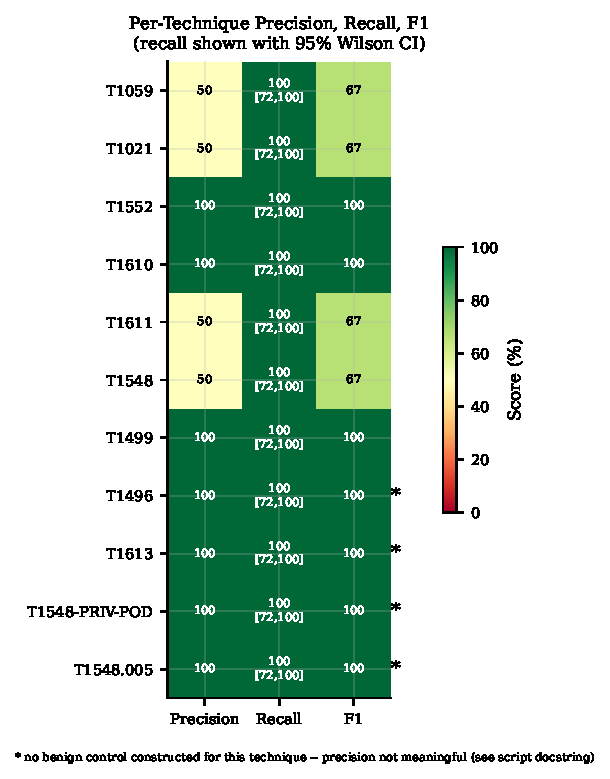
\includegraphics[width=0.85\columnwidth]{fig5_technique_precision_recall_f1.pdf}
\caption{Per-technique precision, recall, and F1-score, with recall's
95\% Wilson confidence interval annotated on each cell. An asterisk
marks the four techniques with no meaningful benign control.}
\label{fig:precision-recall}
\end{figure}

Precision divides the technique set exactly along the design boundary
stated in \S\ref{sec:system-design}. The four techniques with no scope
exclusion (T1059, T1021, T1548, T1611) show precisely 50\% precision,
since each fires on the matched benign action for the same reason it
fires on the attack: a shell spawned during legitimate debugging looks
identical, at the eBPF layer, to one spawned by an attacker, and a
capability check from routine container operation looks identical to
one from privilege escalation or an escape attempt; the exact 50/50
split confirms the benign control was a genuine closest lookalike
rather than exposing an unexpected weakness. The three techniques with
real behavioral discrimination (T1552, T1610, T1499) show 100\%
precision, since their detection logic tests for something a
legitimate action of the same kind does not produce: a secret read
through a compromised service account token, a burst of connections to
several distinct destinations, a burst of process executions well
above routine activity.

This split is a deliberate, disclosed design choice: CAGE favors
recall over precision for the four techniques with no reliable
discriminator, since a missed detection, an attacker already executing
code inside a pod, is costlier than an alert an operator triages and
dismisses. These four rules will therefore false-positive on every
legitimate action of the same shape they catch, at whatever rate that
activity occurs; \S\ref{sec:threat-model} already commits to this
trade-off for T1021, and Table~\ref{tab:per-technique} confirms it
holds, in the same form, for T1059, T1548, and T1611.

Detection latency for these trials falls into three clusters rather
than a single split by source: audit-log-sourced detections and the
Tetragon capability check (T1611) resolve fastest, in 0--4.6 seconds;
T1610 resolves in a distinct middle range, 23.1--23.5 seconds; and the
remaining Tetragon-sourced process-execution techniques (T1059, T1548,
T1499, T1496) resolve in 28.5--29.9 seconds, matching the 27.96-second
mean (95\% CI [27.88, 28.04]) that \S\ref{subsec:rq5} characterizes using T1059
alone at larger scale (N=20), the wider spread here reflecting four
techniques at N=10 each rather than one at N=20. That the same plateau
appears in a correctness experiment never designed to measure latency
is a useful cross-check that the pattern reflects the underlying
telemetry pipeline, not \S\ref{subsec:rq5}'s own methodology.

T1611's speed relative to the other Tetragon-sourced techniques
deserves a note: it detects through a different kernel probe, a
capability check rather than a process-execution event, so its fast
resolution is consistent with, though not confirmed to be caused by,
the connection-age and event-buffering behavior \S\ref{subsec:rq5} reports as
an open question; process-execution events are far more numerous on
this cluster than capability-check events, and a lower-volume event
type would be less exposed to whatever queuing effect produces the
plateau for the busier one. T1610's middle position, faster than the
plateau but slower than an audit-log detection, is consistent with its
dual telemetry path (\S\ref{sec:system-design}): both the Tetragon kprobe and the
independent NetworkMonitor poll feed the same burst-tracking window,
and the alert reflects whichever source completes the threshold
first.

\subsection{RQ2: Cross-Layer Necessity: Telemetry-Source Ablation (E2)}
\label{subsec:rq2}

N=10 trials per technique per condition, 3 conditions
(\texttt{tetragon\_only}, \texttt{audit\_only}, \texttt{fused}), 330 total trials.

\begin{table}[!t]
\centering
\caption{Ablation Study: Detection Rate by Telemetry Configuration.}
\label{tab:ablation}
\tablebodyfont
\begin{tabular}{@{}lccc@{}}
\toprule
\textbf{Technique} & \textbf{Tetragon only} & \textbf{Audit log only} & \textbf{Fused} \\
\midrule
T1059 & 10/10 (100\%) & 0/10 (0\%) & 10/10 (100\%) \\
T1021 & 0/10 (0\%) & 10/10 (100\%) & 10/10 (100\%) \\
T1552 & 0/10 (0\%) & 10/10 (100\%) & 10/10 (100\%) \\
T1610 & 10/10 (100\%) & 0/10 (0\%) & 10/10 (100\%) \\
T1611 & 10/10 (100\%) & 0/10 (0\%) & 10/10 (100\%) \\
T1548 & 10/10 (100\%) & 0/10 (0\%) & 10/10 (100\%) \\
T1496 & 10/10 (100\%) & 0/10 (0\%) & 10/10 (100\%) \\
T1499 & 10/10 (100\%) & 0/10 (0\%) & 10/10 (100\%) \\
T1613 & 0/10 (0\%) & 10/10 (100\%) & 10/10 (100\%) \\
T1548-PRIV-POD & 0/10 (0\%) & 10/10 (100\%) & 10/10 (100\%) \\
T1548.005 & 0/10 (0\%) & 10/10 (100\%) & 10/10 (100\%) \\
\bottomrule
\end{tabular}
\end{table}

Fig.~\ref{fig:ablation-heatmap} renders Table~\ref{tab:ablation} as a heatmap and Fig.~\ref{fig:tactic-radar} as a per-tactic radar
chart, both making the complementary-coverage pattern visually immediate.
This is the paper's central empirical argument for cross-layer fusion.
The split is perfectly complementary with zero exceptions across 220
single-source trials: every technique is detected with 0\% probability
under exactly one single-source condition and 100\% under the other, and
the fused condition recovers 100\% detection across all 11 techniques.

\begin{figure}[!t]
\centering
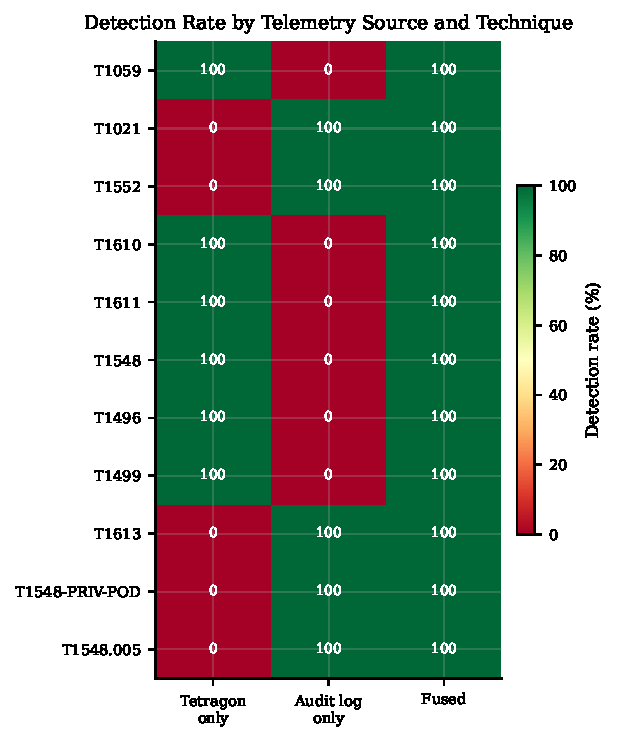
\includegraphics[width=0.85\columnwidth]{fig6_ablation_heatmap.pdf}
\caption{Detection rate by telemetry source and technique, rendered as
a heatmap. Every technique shows 0\% or 100\%, never an intermediate
rate, under each single-source configuration.}
\label{fig:ablation-heatmap}
\end{figure}

\begin{figure}[!t]
\centering
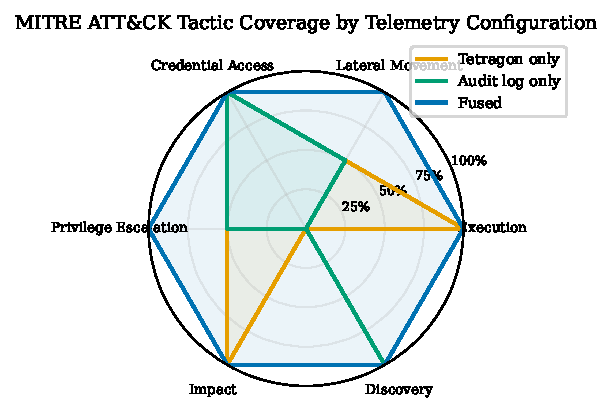
\includegraphics[width=0.85\columnwidth]{fig7_mitre_tactic_radar.pdf}
\caption{MITRE ATT\&CK tactic coverage by telemetry configuration. The
fused configuration's radar envelope fully encloses both single-source
envelopes across every tactic.}
\label{fig:tactic-radar}
\end{figure}

The cleanness of this split, exactly 0\% or exactly 100\%, never a
partial or degraded rate in between, confirms that each technique's
detection logic is implemented entirely on one side of the
eBPF/audit-log boundary, with no rule that partially depends on both
sources to fire; the correlation that spans both sources happens only
at the chain level (\S\ref{subsec:rq3}). A partial rate under ablation
would have signaled an unintended cross-source dependency inside what
was assumed to be a single-source rule; its absence validates the
architecture described in \S\ref{sec:system-design}.

No technique requires \emph{both} sources simultaneously, but no
\emph{single} source covers more than 6 of the 11, so an operator
running either tool alone, regardless of tuning effort, carries a
structural blind spot over roughly half the technique catalog that no
threshold adjustment can close. This is a stronger claim than reduced
sensitivity: the missing techniques are not detected less reliably
under single-source operation, they are categorically undetectable,
since the events they depend on are never produced by the missing
telemetry domain at all, and only restoring the missing source can
recover them. This result directly substantiates the motivating claim
in \S\ref{sec:intro} with controlled, live-cluster measurement rather
than architectural argument alone.

This experiment characterizes complete source removal. It does not
test partial degradation, a telemetry source that is still running but
delayed, dropping events, or intermittently unavailable, which is a
materially different failure mode addressed separately in the
fault-injection evaluation (\S\ref{subsec:rq8}).

\subsection{RQ3: Chain-Correlation Reliability (E3)}
\label{subsec:rq3}

N=10 trials per chain, all 5 documented chains, each trial pair
separated by $>$120s (exceeding the correlation window) to force
genuinely independent episodes, and each chain-type block separated from
the next by the same margin, since several chains share overlapping
trigger actions (\S\ref{sec:lessons} discusses a live-discovered timing pitfall here).
50 total trials, live cluster, current (fixed) episode-scoped dedup
logic.

\begin{table}[!t]
\centering
\caption{Chain Re-Detection Across Independent Episodes.}
\label{tab:chain-dedup}
\tablebodyfont
\begin{tabular}{@{}lc@{}}
\toprule
\textbf{Chain} & \textbf{Fired / N} \\
\midrule
T1059$\to$T1552 & 10/10 \\
T1021$\to$T1059$\to$T1552 & 10/10 \\
T1059$\to$T1610$\to$T1552 & 10/10 \\
T1059$\to$T1548$\to$T1611 & 10/10 \\
T1611$\to$T1552 & 10/10 \\
\bottomrule
\end{tabular}
\end{table}

Fig.~\ref{fig:chain-dedup} plots cumulative detections per trial for a representative chain
against the ideal one-per-trial diagonal, illustrating this reliability
visually alongside the full per-chain breakdown in Table~\ref{tab:chain-dedup}. Every
documented chain re-fires reliably across 10 independent episodes each,
with zero missed detections (50/50).

\begin{figure}[!t]
\centering
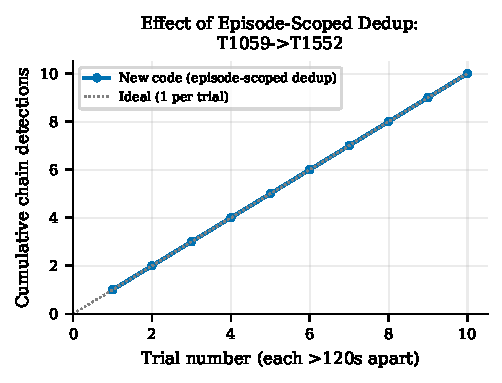
\includegraphics[width=0.88\columnwidth]{fig8_dedup_comparison.pdf}
\caption{Cumulative chain detections per trial for a representative
chain, plotted against the ideal one-detection-per-trial diagonal.}
\label{fig:chain-dedup}
\end{figure}

The methodological choice to space trials more than 120 seconds apart
is what makes this result meaningful rather than trivial. A pod UID
persists for the pod's entire lifetime and is not retired because it
triggered an alert; a real workload can be compromised, remediated,
and compromised again, and each incident needs to be reported
independently. Ten trials fired back to back within the same
120-second window would only demonstrate that a chain can fire once,
since every subsequent trigger would be indistinguishable from the
same ongoing incident by the correlator's own definition; enforcing
genuine separation is what allows 50/50 to be read as evidence the
re-arm mechanism works, not merely that the chain-matching logic
works.

This result also closes the loop on a defect described in \S\ref{sec:lessons}.
The episode-scoped design tested here, retaining a chain's firing key
only while its constituent legs remain continuously satisfied and
discarding it the moment they are not, is the same pattern an earlier
version of the T1499 fork-bomb detector failed to implement: that
detector set its firing key once and never cleared it, so a pod that
triggered it once could never trigger it again. The five chains tested
here already implemented the correct discard-on-condition-false
behavior; this experiment confirms the pattern behaves correctly under
real system conditions and timing, across all five documented chains.
Had the fire-once-forever behavior been present instead, the signature
would be unmistakable: at most the \emph{first} trial of each chain
would have fired, and every subsequent trial against the same
long-lived pod would have registered as a false negative, a defect
signature of precisely 1/10, not the 10/10 observed here.

\S\ref{subsec:rq5} through \S\ref{subsec:rq7} turn to what this correctness costs in
latency, resource overhead, and monitoring scalability; RQ4
(\S\ref{subsec:rq4}) returns to correctness once more to characterize the
one boundary this paper commits to disclosing rather than leaving
implicit.

\subsection{RQ5: Detection Latency (E4)}
\label{subsec:rq5}

Detection latency governs what CAGE's alerts are useful for: an alert
that arrives half a minute late is still evidence, but is no longer a
basis for real-time response, and since CAGE's two telemetry sources
have structurally different delivery paths, one a direct API record,
the other a kernel event surfaced through a kprobe and a
subprocess-mediated read loop, there is no a priori reason to expect
them to behave alike. RQ5 measures this directly rather than assuming
it.

The distribution measurement ran the full plan-specified scale, N=20
trials per technique on the live cluster. Table~\ref{tab:latency} reports the summary
statistics and Fig.~\ref{fig:latency-cdf} plots both techniques' empirical latency
distributions as CDFs, which makes the split between sources visible at
a glance rather than requiring the reader to compare two rows of a
table.

\begin{table}[!t]
\centering
\caption{Detection Latency by Technique and Telemetry Source.}
\label{tab:latency}
\tablebodyfont
\setlength{\tabcolsep}{2.5pt}
\begin{tabular}{@{}llcccccc@{}}
\toprule
\textbf{Tech.} & \textbf{Source} & \textbf{N} & \textbf{Mean (s)} & \textbf{95\% CI (s)} & \textbf{Stdev} & \textbf{Min} & \textbf{Max} \\
\midrule
T1059 & Tetragon eBPF & 20 & 27.96 & [27.88, 28.04] & 0.17 & 27.31 & 28.11 \\
T1552 & K8s audit log & 20 & 0.19 & [0.18, 0.20] & 0.02 & 0.16 & 0.26 \\
\bottomrule
\end{tabular}
\end{table}

Audit-log-sourced detections (T1552) complete in a mean of 0.19
seconds (95\% CI [0.18, 0.20], N=20), consistent with a detection path
that reads a structured record directly from the API server with almost
no intermediate processing. Tetragon-sourced detections (T1059) plateau
at a mean of 27.96 seconds (95\% CI [27.88, 28.04], N=20). The variance
is worth noting on its own terms: a standard deviation of 0.17 seconds
across 20 independent trials is not the signature of an occasional
slow outlier pulling up an average, but a stable, repeatable delay the
eBPF delivery path imposes on every trial alike, on a server that has
been running long enough to leave its initial startup phase behind.

\begin{figure}[!t]
\centering
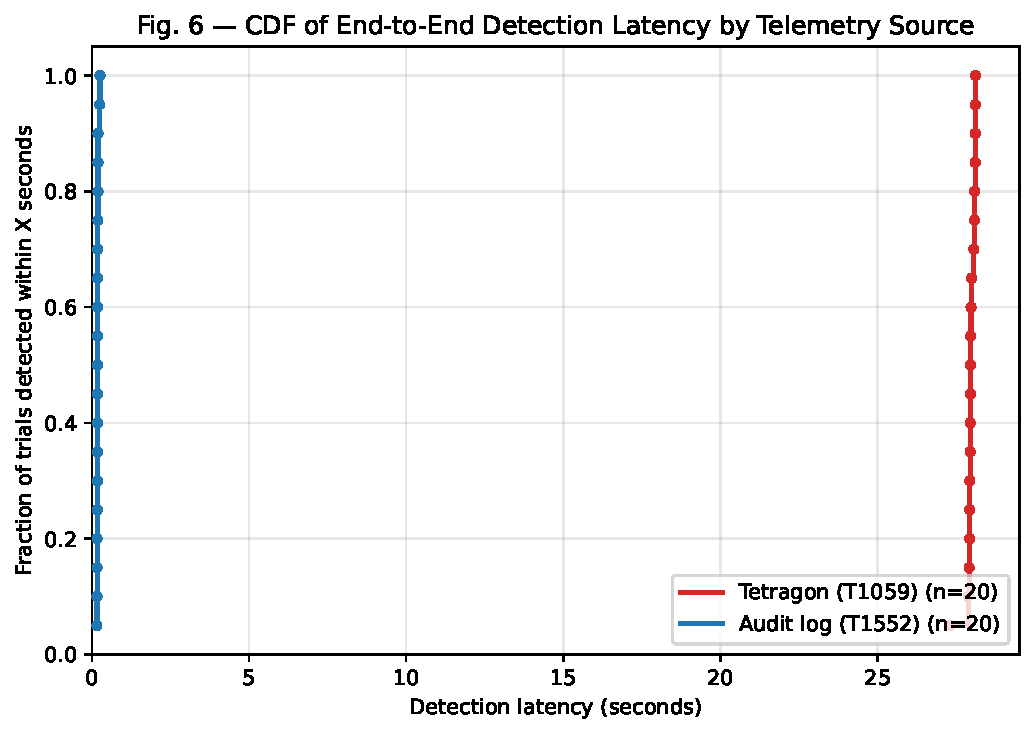
\includegraphics[width=0.88\columnwidth]{fig9_latency_cdf.pdf}
\caption{Cumulative distribution of end-to-end detection latency by
telemetry source (T1059, Tetragon eBPF; T1552, Kubernetes audit log),
N=20 trials each.}
\label{fig:latency-cdf}
\end{figure}

Whether this delay depends on how long the underlying connection has
been open is a question this evaluation could not close, reported as
open rather than forced toward either answer. Two
connection-age sweeps were run, at different scales, using the identical
script and methodology: fire T1059 at controlled elapsed times after a
fresh server restart and record the resulting latency. A pilot-scale
sweep (5 points, ages 7 to 127 seconds) found latency essentially flat
at 29.8 to 30.0 seconds across the entire range, which argued against
age dependence and revised an earlier, less controlled observation that
had suggested younger connections detect faster. A full-scale sweep,
run immediately after the N=20 distribution test, found the opposite
pattern: short, non-monotonic latencies from 0.17 to 14.2 seconds with
no visible trend across the same age range (Fig.~\ref{fig:latency-connage}). These two results
cannot both describe a stable underlying property of connection age, so
one or both must reflect something else. Inspecting the raw server log
for the full-scale run points to a likely explanation: a burst of 13
T1059 detections appears in the 24 seconds immediately following the
sweep's server restart, consistent with a backlog of already-queued
Tetragon events still draining through the newly restarted consumer. The
full-scale sweep followed a 40-detection distribution test, two and a
half times the pilot's event volume, which would plausibly leave a
larger backlog still draining when the sweep's early trials fired and
matched a backlogged detection instead of one the trial itself caused.
This is offered as the most likely explanation supported by the log
evidence, not as a confirmed mechanism, and neither the original
age-dependence hypothesis nor its pilot-scale revision is treated as
settled by this result. \S\ref{sec:limitations} returns to this as a specific,
named limitation rather than a footnote.

\begin{figure}[!t]
\centering
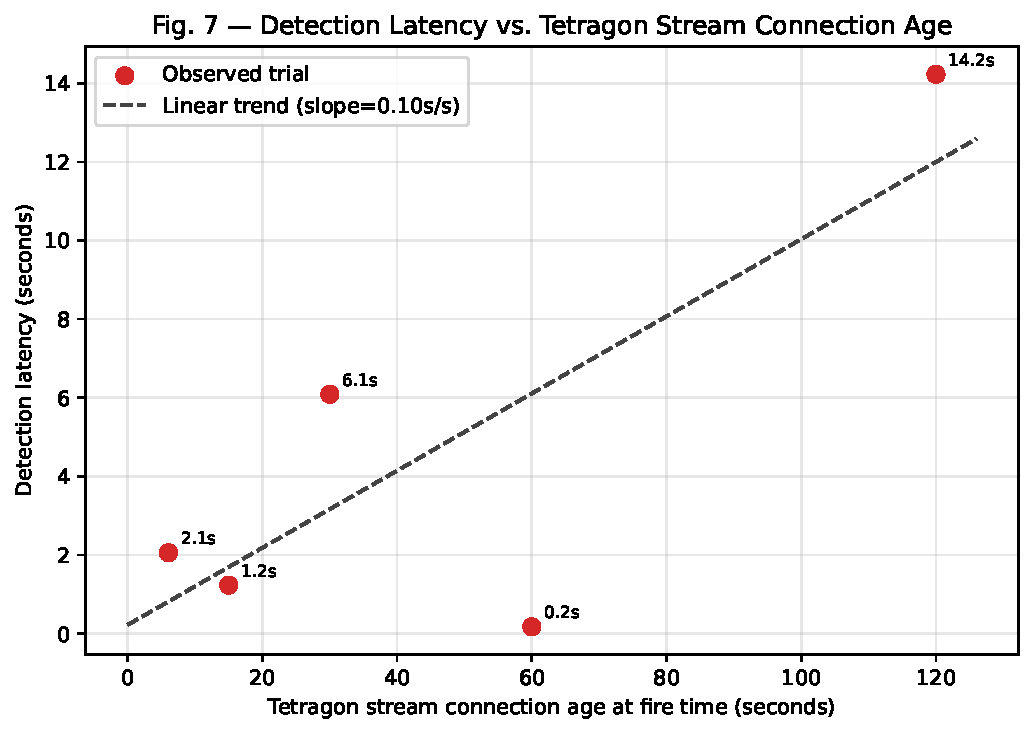
\includegraphics[width=0.88\columnwidth]{fig10_latency_vs_connage.pdf}
\caption{T1059 detection latency versus connection age at the time of
firing, full-scale sweep. No visible trend is present across the
tested age range.}
\label{fig:latency-connage}
\end{figure}

A separate, earlier engineering attempt to reduce this latency by
periodically cycling the Tetragon consumer's underlying subprocess
connection was implemented and tested live against the running system.
It was reverted after introducing measurable event loss without
reliably reducing latency, a cost documented independently of the
connage sweep's own findings and one that would apply regardless of
which explanation for the plateau turns out to be correct.

The practical implication does not depend on resolving the
connection-age question. The N=20 distribution measurement, which
never restarts the server between trials and is therefore not exposed
to the backlog effect described above, is the more reliable basis for
a latency budget: Tetragon-sourced detections should be expected to
complete in roughly 28 seconds, consistently, rather than
near-instantaneously. This is why this evaluation's own scripts use
60-second detection-wait timeouts throughout, and any system consuming
CAGE's alerts downstream should plan for a comparable delay on
eBPF-sourced technique classes, even though audit-log-sourced ones
arrive in a fraction of a second.

\subsection{RQ6: Resource Overhead (E5)}
\label{subsec:rq6}

A detector meant to run continuously on every node has to justify its
own resource cost to the operators it protects, and that cost has to
hold up under real load, not just at idle. RQ6 measures CPU and memory
on the CAGE server process itself across an idle, an active, and a
second idle phase, at the full plan-specified duration: 300 seconds
idle, 600 seconds under a repeating T1059 and T1552 attack load fired
every 3 seconds, and 300 seconds idle again, 241 total samples. Table~\ref{tab:overhead}
reports the phase summary and Fig.~\ref{fig:overhead} plots CPU and RSS across the
full timeline directly.

\begin{table}[!t]
\centering
\caption{Resource Overhead by Phase (CAGE Server Process).}
\label{tab:overhead}
\tablebodyfont
\setlength{\tabcolsep}{2.5pt}
\begin{tabular}{@{}lccccc@{}}
\toprule
\textbf{Phase} & \textbf{N} & \textbf{Mean} & \textbf{95\% CI} & \textbf{Mean} & \textbf{95\% CI} \\
& \textbf{samples} & \textbf{CPU (\%)} & \textbf{CPU (\%)} & \textbf{RSS (MB)} & \textbf{RSS (MB)} \\
\midrule
idle\_pre & 60 & 3.2 & [3.20, 3.20] & 134.8 & [134.80, 134.80] \\
active & 121 & 3.2 & [3.16, 3.18] & 134.8 & [134.83, 134.85] \\
idle\_post & 60 & 3.1 & [3.10, 3.10] & 134.9 & [134.90, 134.90] \\
\bottomrule
\end{tabular}
\end{table}

CPU usage stays within 3.1 to 3.2 percent across all three phases, with
no visible spike when the active phase begins, consistent with the
architecture in \S\ref{sec:system-design}: each event does a fixed,
small amount of work against a bounded per-identity window, so added
event volume does not translate into a larger per-event cost. Memory
tells a similar story: RSS holds between 134.8 and 134.9 megabytes
across the run, growing by roughly 0.1 megabytes over the full 20
minutes. A shorter pilot measurement had left open whether growth of
this kind was bounded or the early part of a slow leak; this longer
window, with five times the active duration and substantially more
accumulated events, resolves that in favor of bounded, consistent with
the periodic stale-pod sweep in \texttt{CausalGraph} reclaiming tracking state
as designed rather than memory accumulating unchecked.

\begin{figure}[!t]
\centering
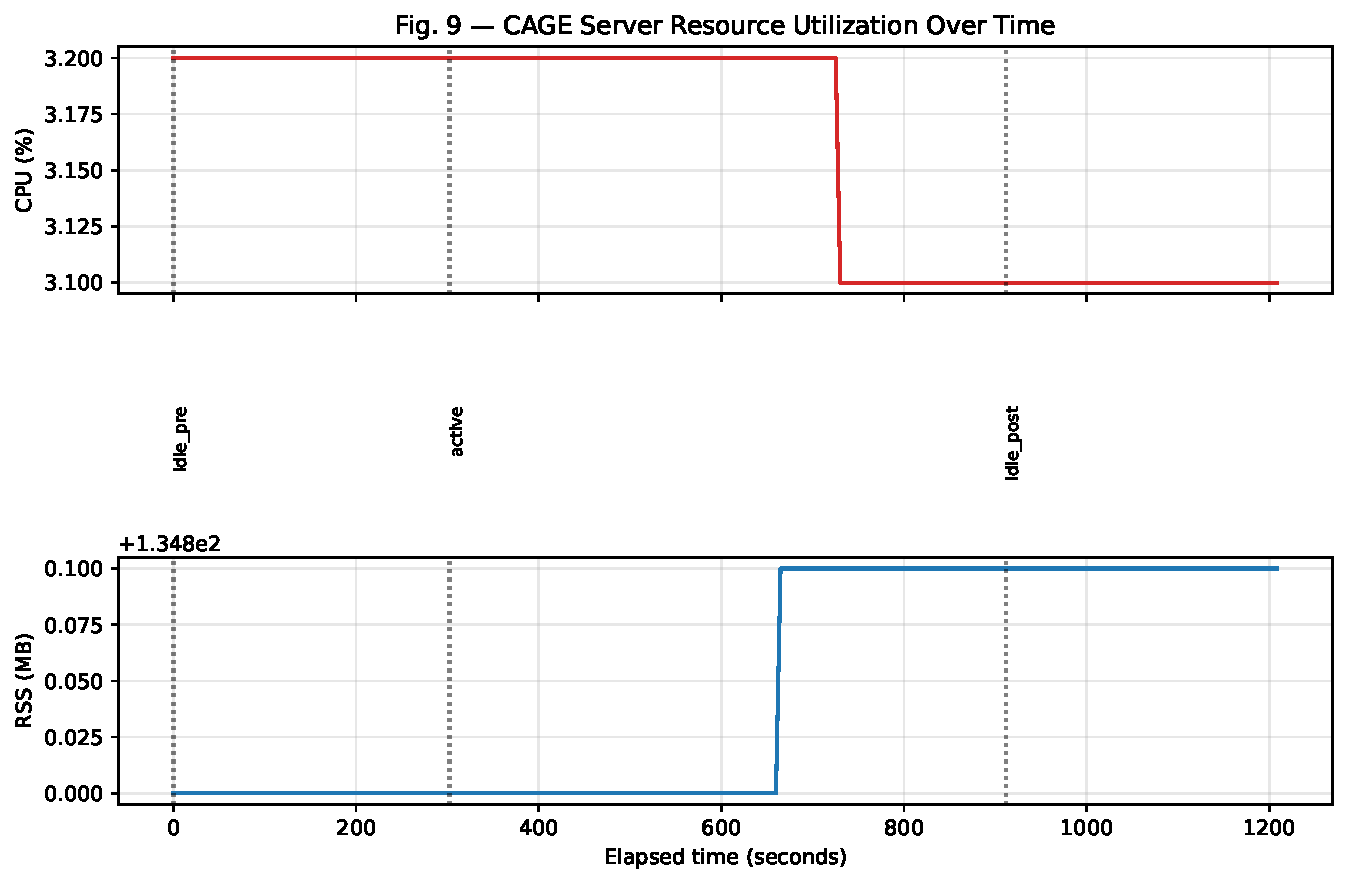
\includegraphics[width=0.88\columnwidth]{fig11_resource_overhead.pdf}
\caption{CPU and resident set size (RSS) of the CAGE server process
across the idle--active--idle timeline. Neither metric shows a visible
step change when the active attack-load phase begins.}
\label{fig:overhead}
\end{figure}

This measurement is scoped deliberately to the CAGE server process
itself: it does not capture Tetragon's own per-node agent cost, since
this \texttt{kind}-based cluster has no metrics-server installed to isolate
that cost separately, a scope limitation carried into
\S\ref{sec:limitations} rather than implied silently. What it does
support is narrower and still useful: CAGE's own correlation layer,
the part of the system this paper's architecture contribution is
about, adds a small, flat cost that does not grow with attack
activity.

\subsection{RQ7: NetworkMonitor Polling Scalability (E6)}
\label{subsec:rq7}

Kubernetes clusters are elastic, and a monitoring component whose
timing degrades as pod count grows can create a detection gap
unrelated to any rule being wrong. RQ7 asks whether that happens to
CAGE's network monitor, and the answer ties directly to a real defect
this project found and fixed during its own development.

The original \texttt{NetworkMonitor} design polled monitored pods
sequentially, one \texttt{kubectl exec} call at a time; this
evaluation's own planning expected cycle time to grow roughly linearly
with pod count, crossing the nominal 5-second target between 5 and 10
pods. That expectation undersold the actual failure mode: with enough
monitored pods, one full sequential sweep could take longer than the
10-second window the T1610 check uses to detect a scan burst, so a
genuine multi-pod scan could split across two sweeps and never
accumulate enough distinct destinations in either window to cross the
threshold, a false negative produced entirely by the monitor's own
polling cadence, discovered while debugging why a real T1610 burst was
not firing rather than a limitation of the detection rule itself. The
fix replaced sequential polling with a \texttt{ThreadPoolExecutor}-based
concurrent sweep, bounding cycle time by the slowest single \texttt{kubectl
exec} call rather than their sum.

Table~\ref{tab:scalability} reports the full-scale measurement of that fix: N in
\{1, 2, 4, 8, 16\} scan-target pods, corresponding to 3 to 18 total
monitored pods, 9 usable inter-wave gaps sampled at each N.

\begin{table}[!t]
\centering
\caption{NetworkMonitor Cycle Time vs.\ Monitored-Pod Count.}
\label{tab:scalability}
\tablebodyfont
\begin{tabular}{@{}ccccc@{}}
\toprule
\textbf{N scan} & \textbf{Total} & \textbf{Waves} & \textbf{Mean} & \textbf{95\% CI} \\
\textbf{targets} & \textbf{monitored} & & \textbf{cycle (s)} & \textbf{(s)} \\
\midrule
1 & 3 & 9 & 4.69 & [3.58, 5.80] \\
2 & 4 & 9 & 4.68 & [3.60, 5.76] \\
4 & 6 & 9 & 5.35 & [4.57, 6.12] \\
8 & 10 & 9 & 5.35 & [4.57, 6.13] \\
16 & 18 & 9 & 4.90 & [3.78, 6.03] \\
\bottomrule
\end{tabular}
\end{table}

Mean cycle time stays within a narrow band, 4.68 to 5.35 seconds,
across the entire tested range, and the 95\% confidence intervals at
every N overlap heavily, all falling roughly within 3.6 to 6.1 seconds.
Two of the five N values have a mean just above the nominal 5-second
target, but given how much the intervals overlap, this reads as noise
around a flat cycle time rather than a genuine upward trend with pod
count, a meaningfully different claim than originally anticipated:
rather than characterizing where a scalability limitation appears,
this result is direct evidence the concurrency fix removed the growth
trend the sequential design would have produced, holding cycle time
flat across an order-of-magnitude range in monitored-pod count.

\subsection{RQ4: Evasion Boundary Characterization (E9)}
\label{subsec:rq4}

N=10 trials per boundary per technique, default thresholds, live
cluster. This experiment answers RQ4 directly; it is a fixed-threshold
boundary characterization, distinct from a full multi-value threshold
\emph{sweep} (varying the threshold itself across several values), which was
explicitly descoped from this evaluation cycle for time (\S\ref{sec:limitations}).

For T1610 and T1613, ``just under'' is exactly one unit below the
documented default threshold; for T1499, ``just under'' uses a
deliberately wider margin (15 versus the threshold of 25) rather than
exactly 24, for a reason reported honestly rather than concealed: live
measurement of the exact per-invocation process-count overhead of the
attack-firing helper proved unreliable across repeated, carefully-spaced
trials, and a defensible-but-imprecise boundary claim was judged
preferable to an exact-sounding one the evidence did not actually
support (\S\ref{sec:lessons}).

\begin{table}[!t]
\centering
\caption{Evasion Boundary Results, Default Thresholds.}
\label{tab:evasion}
\tablebodyfont
\begin{tabular}{@{}lcc@{}}
\toprule
\textbf{Technique} & \textbf{Just under threshold} & \textbf{At threshold} \\
\midrule
T1610 (threshold 5) & 0/10 fired & 10/10 fired \\
T1499 (threshold 25) & 0/10 fired & 10/10 fired \\
T1613 (threshold 10) & 0/10 fired & 10/10 fired \\
\bottomrule
\end{tabular}
\end{table}

Fig.~\ref{fig:evasion-boundary} plots this boundary as a per-technique dot plot, both boundary
conditions shown side by side. All three threshold-based detectors show
the same clean pattern: an attacker who knows the default threshold and
stays under it evades detection with certainty (0/10 across 30 total
sub-threshold trials), while an attacker who reaches the threshold is
caught with equal certainty (10/10 across 30 total at-threshold
trials).

\begin{figure}[!t]
\centering
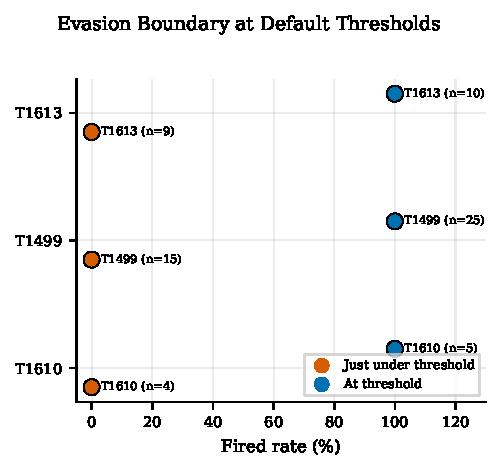
\includegraphics[width=0.85\columnwidth]{fig12_parameter_sensitivity.pdf}
\caption{Evasion-boundary outcomes for T1610, T1499, and T1613 at their
default thresholds: fired rate just under versus at the documented
threshold.}
\label{fig:evasion-boundary}
\end{figure}

The sharpness of this transition, a deterministic 0/10 on one side and
10/10 on the other with no intermediate behavior, confirms that these
three rules are exactly what \S\ref{sec:system-design} describes: fixed
numeric comparisons against a disclosed threshold, not statistical or
learned decision boundaries that would show ambiguous outcomes near
the edge. This is the direct empirical counterpart to the trade-off
argued architecturally in \S\ref{sec:system-design}: CAGE's
bounded-window, rule-based approach cannot generalize beyond its
explicit rule set, but in exchange produces alerts that trace to one
named rule and one disclosed threshold rather than a boundary that
depends on training data, a trade-off RQ4 makes concrete instead of
asserted.

We report this as a measured, disclosed property of a threshold-based
detector (\S\ref{sec:threat-model}) rather than a weakness discovered
post hoc; the threat model already scopes this boundary as known and
deliberately characterized, and this experiment is that
characterization. The practical implication is narrower than it might
first appear: it establishes where the boundary sits, not what happens
to detection and false-positive rates at any other threshold value.
Lowering a threshold to catch a more cautious attacker is the only
lever available for these three rules, trading directly against false
positives on legitimate bursty behavior of the same shape, a burst of
routine connections, executions, or RBAC reads. Characterizing that
trade-off across the full range of threshold values, rather than only
at the default and its immediate boundary, is the threshold-sweep
experiment descoped for time in this evaluation cycle
(\S\ref{sec:limitations}) and remains open work.

\subsection{RQ8: Fault Injection and Recovery (E8)}
\label{subsec:rq8}

CAGE's threat model treats its own process as trusted but the
infrastructure it depends on, the kernel agent, the audit log, the API
server, as fallible in ordinary, non-adversarial ways: containers
restart, files get truncated, control planes have bad days. RQ8 tests
whether the reconnect, backoff, and retry logic already present in the
codebase actually delivers on that resilience claim when the
underlying infrastructure genuinely fails, rather than only in
description.

Three faults were injected against the live, fully fused server, in
ascending order of severity. The first kills the local \texttt{tetra getevents}
subprocess directly, exercising the Tetragon consumer's own 2-second
self-healing reconnect loop. The second truncates the Kubernetes audit
log to zero bytes in place, exercising \texttt{tail -F --retry}'s handling of
truncation specifically, a different failure mode from the log rotation
the same flag also has to survive. The third stops and restarts the
entire \texttt{cage-control-plane} container, removing the API server, that
node's Tetragon agent, and the audit log file all at once, the most
severe single fault tested here. Each scenario ran 5 independent
repetitions, 15 fault injections in total. Fig.~\ref{fig:fault-timeline} shows a representative
recovery timeline across all three, and Table~\ref{tab:fault-recovery} reports the
aggregated result per scenario with a Wilson 95\% confidence interval on
the recovery rate.

\begin{table}[!t]
\centering
\caption{Fault-Recovery Outcome by Scenario (Wilson 95\% CI).}
\label{tab:fault-recovery}
\tablebodyfont
\begin{tabular}{@{}lcccc@{}}
\toprule
\textbf{Scenario} & \textbf{Reps} & \textbf{Functional} & \textbf{Wilson} & \textbf{Spurious} \\
& & \textbf{recovery} & \textbf{95\% CI} & \textbf{alerts} \\
\midrule
tetragon-consumer-kill & 5 & 5/5 (100\%) & [0.57, 1.00] & 4 \\
audit-log-truncate & 5 & 5/5 (100\%) & [0.57, 1.00] & 12 \\
control-plane-outage & 5 & 5/5 (100\%) & [0.57, 1.00] & 0 \\
\bottomrule
\end{tabular}
\end{table}

All 15 injected faults recovered functionally, meaning a real
post-fault attack was fired and correctly detected, without manual
intervention: 5 out of 5 for every scenario, Wilson 95\% CI [0.57, 1.00]
in each case. That interval's lower bound sits well below 1.0 despite
every trial succeeding: at a sample size of 5, a perfect result is
still compatible with a true recovery rate as low as 0.57, so
reporting the interval alongside the point estimate keeps that
uncertainty visible rather than implying a stronger guarantee than
five trials can support. Mean functional-recovery time was 13.3
seconds for the Tetragon-kill scenario, 226.0 for the audit-log
truncation, and 250.3 for the control-plane outage, the same ordering
a smaller pilot run found earlier (34.9, 241.9, and 303.8 seconds
respectively), with the full-scale means somewhat faster, plausibly
because the pilot's single control-plane trial caught extra apiserver
warmup variance that averages out across five repetitions. None of
the recovery mechanisms exercised here, the Tetragon consumer's
reconnect loop, the pod UID cache's exponential backoff, \texttt{tail
-F --retry}'s own truncation handling, were written for this
experiment; all three are pre-existing production code tested here
under real failure, not logic added to pass it.

\begin{figure}[!t]
\centering
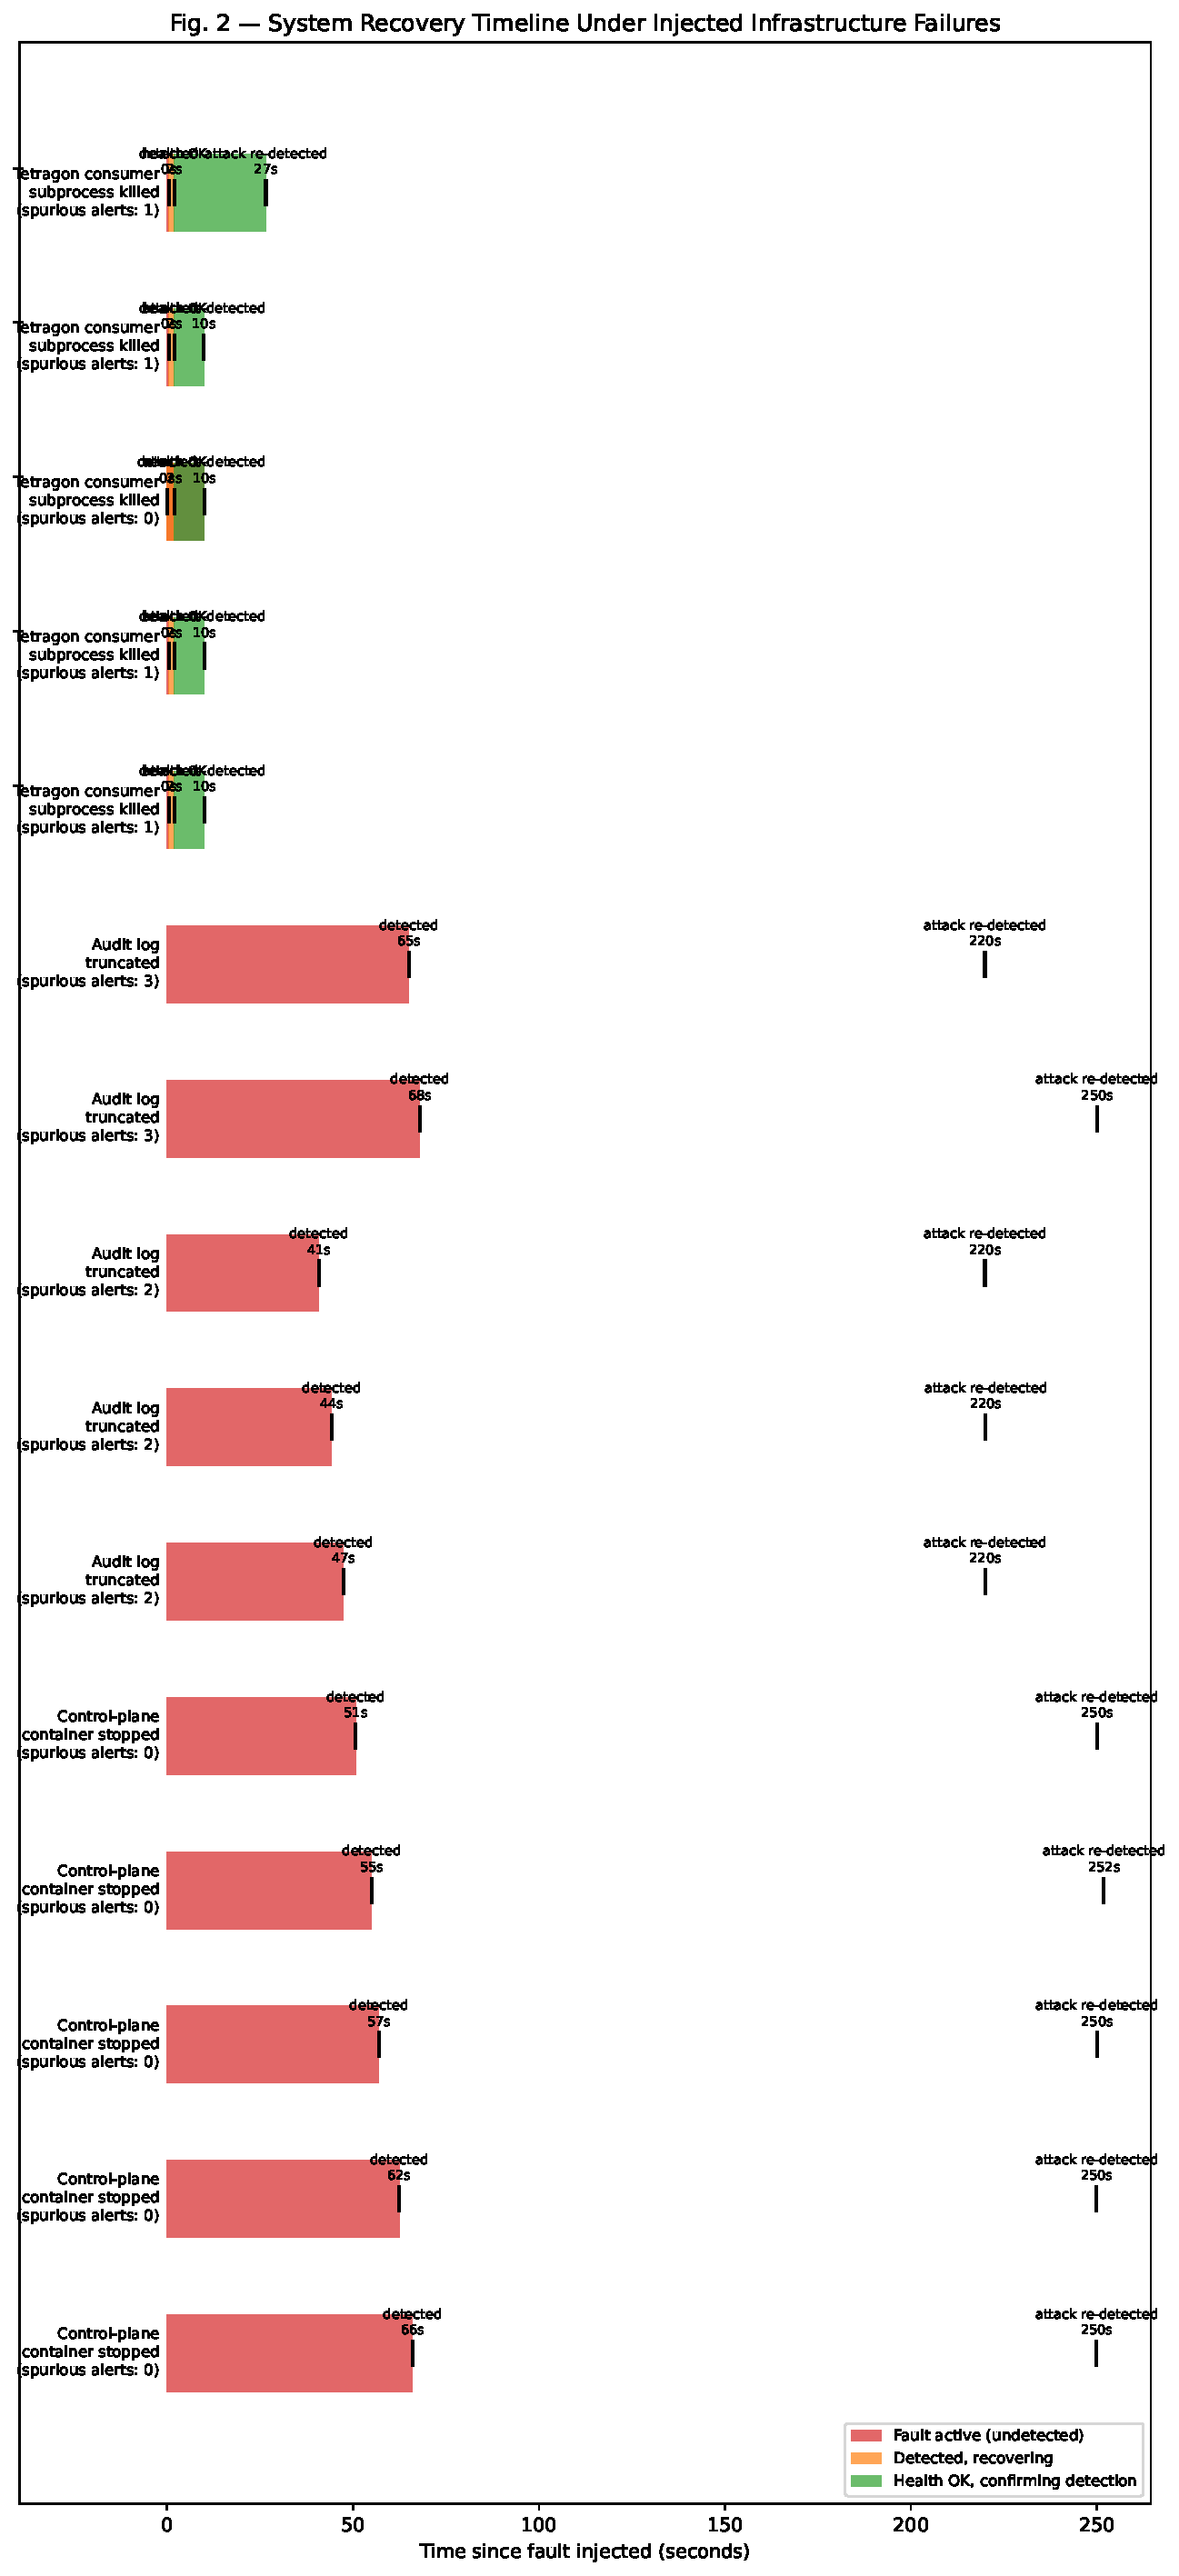
\includegraphics[width=0.72\columnwidth]{fig13_fault_recovery_timeline.pdf}
\caption{Representative recovery timeline across the three injected
fault scenarios (Tetragon-consumer kill, audit-log truncation,
control-plane outage), showing fault onset, health-flag recovery, and
functional recovery.}
\label{fig:fault-timeline}
\end{figure}

Spurious alerts during the fault windows were uneven across scenarios:
4 total across the 5 Tetragon-kill windows, 12 across the 5 audit-log
truncation windows, and none across the 5 control-plane windows. This
pattern tracks window duration rather than suggesting fault-induced
false positives: the attacker pod's own background loop fires a
legitimate T1059 roughly every 30 seconds regardless of any fault
tested, and the audit-truncate and control-plane scenarios both have
functional-recovery windows lasting several minutes, giving that loop
more opportunities to land inside the window than the short
Tetragon-kill scenario. This evaluation did not isolate that
background activity with a dedicated no-traffic control run, needed to
rule out fault-induced false positives with certainty rather than by
inference from timing; that gap is carried into \S\ref{sec:limitations}
as a named limitation.

A secondary result concerns the \texttt{/api/health} staleness flag
rather than the faults themselves. For two of the three scenarios,
health-recovery could not be read directly off that flag, since it
only clears when a new event arrives and no incidental traffic
occurred between fault resolution and the deliberate recovery attack.
This is precisely why functional recovery, firing a real attack and
confirming detection, is this experiment's primary claim rather than
the health flag's own state: a flag updating only on new traffic
cannot, by construction, prove recovery before something generates
that traffic. It also validates a specific design choice from
\S\ref{sec:system-design}, keeping health observability separate from
the detection path; had the two been coupled, this experiment would
have had no independent way to distinguish an infrastructure problem
from a detection problem.

\section{Lessons from Live-System Evaluation}
\label{sec:lessons}

The results in \S\ref{sec:results} describe what CAGE detects and what that
detection costs; this section describes something different: what
building and evaluating CAGE against real, running infrastructure
taught us about designing and testing systems of this kind. Two people
evaluated two structurally different halves of the same codebase in
parallel, one testing detection logic, the other testing systems
behavior, and each surfaced real defects the other never encountered
and neither anticipated in advance, a pattern the specific lessons
below develop.

\textbf{Fusing two telemetry domains requires a shared vocabulary, not
just two working consumers.} Tetragon events describe a binary, its
arguments, and its process lineage; audit records describe a verb, a
resource, and a requesting identity. Running both consumers correctly
was not sufficient for the correlation this paper's architecture
depends on; each had to be rewritten into one common event shape
before a single chain rule could test them together, since a system
that instruments two sources without this normalization step sees
everything CAGE sees but has no way to reason about it as one
incident.

\textbf{Correlation state tied to a Kubernetes-native identity needs to
re-arm, not just match.} A pod UID is not retired when it triggers an
alert; it can persist for a workload's entire operational lifetime,
compromised and remediated more than once. An earlier version of the
fork-bomb detector treated its firing key as permanent, so a pod that
triggered it once could never trigger it again, not a matching-logic
error but an implicit assumption that firing once was the end of the
story. The fix generalizes: any correlation state keyed to a
long-lived, reusable identifier needs an explicit condition for
clearing itself, or it silently degrades into a permanent allowlist
for exactly the workloads an operator most needs to keep watching.

\textbf{Evaluation tooling fails in ways that have nothing to do with
the system it is testing, and deserves the same scrutiny.} A
metrics-collection script matching alerts to events via a shared
30-second window, rather than each trial's own scoped log region,
would have silently inflated precision for the two techniques whose
design makes them fire unconditionally, exactly where an inflated
number would be least noticeable. Separately, a chain-alert search
pattern written against a literal Unicode arrow failed to match the
system's own ASCII-rendered log output, indistinguishable from a real
detection failure without opening the log directly. Neither defect
lived in the detection logic being measured, yet both would have
produced results that looked complete and internally consistent while
being wrong.

\textbf{Kubernetes deployment realities are a distinct cost from
detection accuracy, and belong in the evaluation, not just the
changelog.} T1610's kprobe-based path depends on a BTF-enabled kernel
not every managed offering exposes; reading the audit log at all
requires patching the API server's own manifest, a step some managed
control planes do not permit; and even inside a fully self-managed
\texttt{kind} cluster, an audit-policy file mounted from a path outside
the repository did not survive cluster recreation. None of these
affect whether a rule fires correctly, but all of them affect whether
the system can be stood up at all in a given environment, a question
detection accuracy cannot answer on its own.

\textbf{A live, multi-hour evaluation needs to survive its own
interruptions, not just produce correct numbers when it finishes
cleanly.} An early version of this evaluation's own scripts wrote
results only once, at completion; a single transient \texttt{kubectl}
timeout partway through an unattended run discarded roughly 35 minutes
of collected data. Writing each trial's result to disk immediately
rather than buffering until the end cost nothing in the common case
and made every subsequent crash recoverable, a starting assumption for
any hours-long unattended run against live infrastructure, not a
lesson learned partway through data collection.

\textbf{A system's own health telemetry is evidence of activity, not
proof of recovery.} CAGE's health endpoint's staleness flag only
clears when a new event actually arrives, so it cannot, by
construction, confirm that a component has recovered before something
generates traffic for it to observe. Resilient reconnect and retry
logic is necessary but does not, by itself, demonstrate that the
resilience works; only firing a real event afterward and confirming it
is still detected does that. Any system that reports its own health
passively should be evaluated by testing what it actually does under
failure, not by reading what it says about itself.

Every defect described here was found by running the system against
live infrastructure and watching it behave unexpectedly, not by
reading code that later turned out to be wrong. Static analysis and
unit tests remain necessary, but neither would have surfaced a dedup
flag that never clears, a matching window that silently misattributes
false positives, or a health flag that cannot prove what it appears to
prove. For systems whose correctness depends on multi-source event
timing, long-lived identity state, and cross-process coordination,
that gap between code review and live behavior is the strongest
argument this paper can make for why systems of this kind should be
evaluated the same way.

\section{Limitations and Threats to Validity}
\label{sec:limitations}

We organize the limitations of this work around four standard
categories: internal validity, whether the causal explanations we
offer for observed behavior are actually correct; external validity,
whether our findings generalize beyond the specific environment we
tested; construct validity, whether our measurements capture what we
intend them to; and reliability, whether the evaluation itself can be
reproduced and trusted.

\subsection{Internal Validity}
\label{subsec:internal-validity}

The Tetragon delivery-latency plateau (\S\ref{subsec:rq5}) is characterized
precisely and reproducibly, a standard deviation of 0.17 seconds
across 20 trials, but its underlying mechanism inside Tetragon's own
event-delivery path was not conclusively identified within this
project's scope: an engineering fix based on one candidate
explanation, periodic subprocess cycling, was implemented, tested
live, and reverted after it traded latency for measurable event loss.
The plateau itself is a solid, repeatable finding; the causal
explanation for why it exists at exactly that duration is not.

Whether this same delay depends on connection age remains genuinely
unresolved, as \S\ref{subsec:rq5} details: the two connection-age
sweeps produced contradictory results, and neither the original
age-dependence hypothesis nor its later revision is treated as
settled. A reader relying on this paper to reason about Tetragon's own
internals, rather than CAGE's behavior, should not treat either as
established.

The T1499 evasion-boundary result (\S\ref{subsec:rq4}) uses a
deliberately wider sub-threshold margin than T1610 and T1613, for the
reason detailed there: the boundary is real and honestly
characterized, but a comfortably-under-threshold point rather than an
exact threshold-minus-one measurement.

The spurious-alert pattern observed during fault injection
(\S\ref{subsec:rq8}) has the same structure as the connection-age
question above: a plausible explanation, tied to background attacker
traffic and each scenario's recovery-window length, supported by
circumstantial timing evidence rather than a dedicated no-traffic
control run, so fault-induced false positives cannot be ruled out with
full certainty.

\subsection{External Validity}
\label{subsec:external-validity}

All experiments ran on a single-control-plane, two-worker \texttt{kind}
cluster inside a WSL2 virtual machine, not a production-scale,
multi-node, bare-metal deployment. Absolute timing numbers, the
roughly 28-second Tetragon plateau specifically, may not transfer
unchanged to bare metal; the relative pattern this paper's argument
depends on, a large and consistent gap between audit-log and
eBPF-sourced detection latency, is the more robust claim we ask
readers to generalize from. Audit-log access itself requires patching
the API server's own manifest, a step not available on every managed
Kubernetes offering, a deployment constraint independent of anything
CAGE's detection logic does.

T1610's kprobe-based detection path requires a BTF-enabled kernel,
confirmed functional on kernel 6.6 but not independently verified
across managed offerings that restrict kernel access, so its
portability outside this specific environment remains an open question
rather than a confirmed capability.

Every attack in this evaluation is a fixed, disclosed, non-adaptive
command sequence, run exactly as documented, so the detection numbers
in \S\ref{sec:results} characterize CAGE's behavior against this specific,
published attack set, not robustness against an adversary actively
trying to evade these exact rules, beyond the one boundary this paper
deliberately measures in \S\ref{subsec:rq4}. The single real evasion
vector found during this project, a name-based scope exclusion that
would have let an attacker rename a pod to suppress its own detection,
was found incidentally during development, not through systematic
red-teaming, and was fixed before any evaluation data was collected on
it. That it was found by accident rather than by deliberate search
makes an unknown number of similar vectors plausible, not just the two
named here; timing fragmentation across the 120-second correlation
window and binary renaming are the two we can name in advance, not an
exhaustive list of what remains untested.

This paper's comparison against related systems (Table~\ref{tab:related-work}) is
qualitative, built from each system's own published description rather
than a controlled, head-to-head measurement. The cheapest and
highest-value quantitative addition, running vanilla Tetragon against
the same attack set used in \S\ref{subsec:rq1} and \S\ref{subsec:rq2}, remains future work
rather than a claim this paper makes.

\subsection{Construct Validity}
\label{subsec:construct-validity}

T1021 carries no scope exclusion at all, by deliberate design
(\S\ref{sec:system-design}), flagging every \texttt{kubectl exec} including
routine administrative access. This is a disclosed precision cost, not
an oversight, but it means the 50 percent precision reported for T1021
in Table~\ref{tab:per-technique} measures the rate against this
evaluation's specific benign-control workload, not the baseline rate
of legitimate \texttt{kubectl exec} traffic any particular production
cluster would see; a cluster with substantially more or less routine
exec activity than our benign control would observe a different
precision number without any change to CAGE's own logic.

Detection-quality experiments use N=10 trials per condition
(\S\ref{sec:eval-methodology}), a resource-bounded choice rather than
an arbitrary one, which narrows the 95 percent Wilson confidence
interval to a floor of 72.2 percent even where every trial succeeded.
We report confidence intervals throughout specifically so this
constraint stays visible to the reader rather than hidden behind point
estimates.

\subsection{Reliability and Reproducibility}
\label{subsec:reliability}

Two experiments planned for this evaluation cycle were explicitly
descoped for time: a direct old-code-versus-new-code comparison
isolating the chain-correlation dedup fix, and a full multi-value
threshold sweep rather than only a default-versus-boundary comparison.
Neither affects the validity of the results reported; both would add
depth to \S\ref{subsec:rq3} and \S\ref{subsec:rq4} as concrete,
well-scoped future work.

The evaluation infrastructure itself was not free of defects:
\S\ref{sec:lessons} documents several real bugs found only by running
this evaluation against live infrastructure, a metrics-matching window
that could have misattributed false positives, a string-matching
pattern that could have masked real detections, and
process-identification bugs that corrupted two full-scale systems
measurements before being caught and fixed. We report this directly,
rather than as an embarrassment to minimize, because it is a property
of the evaluation environment anyone extending this work should know
about, and because catching and correcting it is itself part of what
this paper's methodology demonstrates.

Finally, CAGE's own runtime credentials in this evaluation are broader
than its architecture requires: as \S\ref{sec:threat-model} discloses, CAGE
authenticates with the same local kubeconfig used to administer the
cluster rather than a purpose-built, minimally-scoped ServiceAccount,
even though its actual behavior is read-only by design. This does not
affect any finding in this paper, since CAGE's own process was never
adversarially targeted, but it is a real gap between what a production
deployment should grant and what this evaluation environment granted,
reported here as future hardening work rather than left undisclosed.

\section{Conclusion}
\label{sec:conclusion}

Two telemetry domains already exist inside every Kubernetes cluster
that runs eBPF-based monitoring alongside the API server's own audit
log, and neither one is looking at the other. That gap is not a
tooling oversight; it follows directly from what each domain can
observe on its own. A shell spawned inside a container and the
\texttt{kubectl exec} session that opened it are two halves of one action,
visible to two different instruments, and nothing in either instrument
knows the other half exists. CAGE's contribution is not the general
idea of fusing kernel-level and control-plane telemetry, since
provenance- and correlation-based systems adjacent to this problem
already exist, but none of them actually combines these two specific
sources; each sits on only one side of the boundary this paper
addresses. CAGE's contribution is the specific mechanism that makes
that combination trustworthy: resolving the Kubernetes pod UID
reliably from an eBPF event stream that learns about container
identity on a different schedule than the audit log does, and holding
that identity steady enough that a technique detected by one source
and a technique detected by the other can be attributed, with
confidence, to the same running workload.

The evaluation in this paper tests that claim from several independent
angles rather than asserting it once. The ablation study showed a
detection split with no partial cases, every technique detected with
certainty under exactly one single-source configuration and the other,
a stronger result than reduced sensitivity would have been: the
missing techniques under single-source operation are not weakly
detected, they are structurally undetectable. The chain-correlation
experiment showed the same episode-scoped design holding up across ten
independently spaced incidents per chain, on the same long-lived pod
identity, the condition under which a naive, fire-once deduplication
scheme would have failed silently after its first trial. The
evasion-boundary experiment showed that CAGE's threshold-based
detectors behave exactly as their disclosed design says they should, a
deterministic line rather than a probabilistic one. None of these
three results depend on the other two, and together they describe one
consistent design posture: CAGE gives up the generality a learned or
graph-based detector could offer in exchange for behavior that is
fully disclosed and traceable to one named rule.

That posture would be a weak trade if it were expensive to run. It is
not: the same live cluster that produced the detection results also
showed CPU and memory holding flat under active attack load rather
than growing with event volume, a monitoring subsystem whose cycle
time stayed within a narrow band across an order-of-magnitude range in
monitored-pod count once a concurrency defect in its original design
was corrected, and functional recovery from every one of fifteen
injected infrastructure faults without an operator stepping in. A
detector that is accurate but unpredictable under load, or resilient
in description but untested against a real failure, would not answer
the question this paper set out to answer; reporting both halves
against the same infrastructure, rather than treating accuracy and
deployability as separate studies, is what lets this paper make a
claim neither half could support alone.

One further finding sits outside any single research question: as
\S\ref{sec:lessons} details, two people evaluating two different halves
of this same codebase each surfaced real defects that static analysis
had missed and that the other evaluator never encountered, none of
them adversarial, all found only once the system ran against live
infrastructure. That pattern is not specific to CAGE: any system whose
correctness depends on cross-process state and multi-source event
timing carries the same risk, and this paper's experience argues that
such systems need to be evaluated the same way.

This evaluation also has real limits on what it can claim, detailed
fully in \S\ref{sec:limitations}: every number here comes from a
single-host, two-worker cluster, so the relative audit-log-versus-eBPF
latency gap is the more robust claim to generalize from than the
absolute 28-second plateau; every attack was fixed and disclosed
rather than adversarially adaptive, beyond the one threshold boundary
measured directly in \S\ref{subsec:rq4}; and the comparison against
related systems in Table~\ref{tab:related-work} remains qualitative
rather than a controlled, same-cluster measurement.

Three directions follow from what this implementation already puts in
place, rather than from a wish list assembled after the fact. The
ablation infrastructure built for RQ2 already runs CAGE in a
\texttt{tetragon\_only} configuration; pointing that same configuration,
unmodified, at a plain vanilla-Tetragon deployment against the same
attack set used in this evaluation would turn
Table~\ref{tab:related-work}'s qualitative comparison into a direct,
quantitative one at comparatively little additional engineering cost,
since the infrastructure this would require already runs in this
project's cluster. Extending the pod-UID correlation key across
cluster boundaries is a second concrete step: folding a cluster
identifier into the correlation key and watching more than one API
server concurrently, neither of which the current design attempts.
Third, the Tetragon-sourced latency plateau is characterized here with
considerable precision but without a confirmed mechanism; tracing it
to a specific stage inside Tetragon's own event-delivery path, rather
than inferring it indirectly through server-side timing as this
evaluation did, is a well-scoped systems investigation that the
current results motivate directly.

Reduced to its essential claim, this paper shows that fusing kernel-level
and control-plane telemetry in Kubernetes is not primarily a matter of
running two collectors side by side. It depends on resolving one
identity reliably across two sources that disagree about how quickly
that identity becomes known, and once that problem is solved
correctly, the detection gap that motivated this work closes
structurally rather than incrementally, at a cost this paper measured
rather than assumed. That identity-resolution problem is not unique to
the two sources examined here, and the architecture built to solve it
in this paper is offered as a pattern other cross-layer runtime
security systems can reuse, not only as a description of what CAGE
itself does.

\begin{thebibliography}{00}

\bibitem{ref1} The Falco Project, Cloud Native Computing Foundation. [Online]. Available: \url{https://falco.org/}

\bibitem{ref2} Cilium Tetragon, Cilium project / Isovalent. [Online]. Available: \url{https://tetragon.io/}

\bibitem{ref3} M. Franzil, V. Armani, L. A. Dias Knob, and D. Siracusa, ``Sharpening
Kubernetes audit logs with context awareness,'' \emph{Computer Networks}, vol.
276, art. no. 111890, Feb. 2026, doi: 10.1016/j.comnet.2025.111890.

\bibitem{ref4} M. Abbas, S. Khan, A. Monum, F. Zaffar, R. Tahir, D. Eyers, H.
Irshad, A. Gehani, V. Yegneswaran, and T. Pasquier, ``PACED:
Provenance-based automated container escape detection,'' in \emph{Proc. 2022
IEEE Int. Conf. Cloud Eng. (IC2E)}, San Francisco, CA, USA, Apr. 2022,
pp. 261--272.

\bibitem{ref5} X. Han, T. Pasquier, A. Bates, J. Mickens, and M. Seltzer, ``UNICORN:
Runtime provenance-based detector for advanced persistent threats,'' in
\emph{Proc. Network and Distributed System Security Symp. (NDSS)}, San Diego,
CA, USA, Feb. 2020.

\bibitem{ref6} Red Hat, ``The state of Kubernetes security report: 2024 edition,''
Red Hat, Inc., 2024. [Online]. Available: \url{https://www.redhat.com/en/engage/state-kubernetes-security-report-2024}

\bibitem{ref7} Wiz Research, ``Kubernetes Security Report 2025,'' Wiz, Inc., 2025.
[Online]. Available: \url{https://www.wiz.io/reports/kubernetes-security-report-2025}

\bibitem{ref8} O. Bajaber, B. Ji, and P. Gao, ``P4Control: Line-rate cross-host
attack prevention via in-network information flow control enabled by
programmable switches and eBPF,'' in \emph{Proc. 2024 IEEE Symp. Security and
Privacy (S\&P)}, San Francisco, CA, USA, May 2024.

\bibitem{ref9} MITRE Corporation, ``MITRE ATT\&CK.'' [Online]. Available:
\url{https://attack.mitre.org/}. Accessed: Jul. 27, 2026.

\bibitem{ref10} S. Roy, E. Panaousis, C. Noakes, A. Laszka, S. Panda, and G.
Loukas, ``SoK: The MITRE ATT\&CK framework in research and practice,''
arXiv preprint arXiv:2304.07411, 2023.

\bibitem{ref11} S. Ghimire, N. Bhurtel, R. Sahani, and S. Jha, ``eBPF-PATROL:
Protective agent for threat recognition and overreach limitation using
extended Berkeley Packet Filter (eBPF) in containerized and virtualized
environments,'' arXiv preprint arXiv:2511.18155, 2025.

\bibitem{ref12} Z. Cheng, Q. Lv, J. Liang, Y. Wang, D. Sun, T. Pasquier, and X.
Han, ``KAIROS: Practical intrusion detection and investigation using
whole-system provenance,'' in \emph{Proc. 2024 IEEE Symp. Security and
Privacy (S\&P)}, San Francisco, CA, USA, May 2024, pp. 3533--3551.

\bibitem{ref13} F. Wilkens, F. Ortmann, S. Haas, M. Vallentin, and M. Fischer,
``Multi-stage attack detection via kill chain state machines,'' in \emph{Proc.
3rd Workshop on Cyber-Security Arms Race (CYSARM '21)}, Virtual Event,
Republic of Korea, Nov. 2021, pp. 13--24.

\bibitem{ref14} E. B. Wilson, ``Probable inference, the law of succession, and
statistical inference,'' \emph{J. Amer. Statist. Assoc.}, vol. 22, no. 158,
pp. 209--212, 1927.

\bibitem{ref15} O. Jarkas, R. Ko, N. Dong, and R. Mahmud, ``A container security
survey: Exploits, attacks, and defenses,'' \emph{ACM Comput. Surv.}, vol.
57, no. 7, pp. 1--36, Feb. 2025, doi: 10.1145/3715001.

\bibitem{ref16} Kubernetes, Cloud Native Computing Foundation. [Online].
Available: \url{https://kubernetes.io/}

\bibitem{ref17} eBPF, Linux Foundation. [Online]. Available: \url{https://ebpf.io/}

\bibitem{ref18} E. M. Hutchins, M. J. Cloppert, and R. M. Amin, ``Intelligence-driven
computer network defense informed by analysis of adversary campaigns
and intrusion kill chains,'' \emph{Leading Issues Inf. Warfare Secur. Res.},
vol. 1, no. 1, p. 80, 2011.

\end{thebibliography}

\appendices
\section{Reproducibility Artifacts}
\label{app:reproducibility}

\textbf{Repository organization.} Detection-quality experiments (E1, E2,
E3, E9; \S\ref{subsec:rq1}, \S\ref{subsec:rq2}, \S\ref{subsec:rq3}, \S\ref{subsec:rq4}), their scripts, and their raw data
live under \url{evaluation/person_a/}; systems-characteristics experiments
(E4, E5, E6, E8; \S\ref{subsec:rq5}, \S\ref{subsec:rq6}, \S\ref{subsec:rq7}, \S\ref{subsec:rq8}) live under
\url{evaluation/person_b/}. Each directory's own \texttt{README.md} gives the
exact run order and command-line invocations used to produce the
results in this paper. \texttt{restart\_cage.sh} (repository root) rebuilds
the evaluation environment, the \texttt{kind} cluster, Tetragon, and the
audit-log-patched API server, from a clean state.

\textbf{Datasets.} Table~\ref{tab:artifacts} lists the raw CSV file backing each result
table and figure in \S\ref{sec:results}, along with its row count. Every experiment's
trial-level data is preserved exactly as collected; no CSV is
regenerated or overwritten between the pilot-scale and full-scale
runs, and pilot-scale files are kept alongside the full-scale ones
(\url{evaluation/person_b/data/*_pilot_*.csv},
\url{evaluation/person_a/output_pilot_N2-3/}) for direct comparison.

\begin{table}[!t]
\centering
\caption{Raw CSV Files and What They Back.}
\label{tab:artifacts}
\tablebodyfont
\setlength{\tabcolsep}{2.5pt}
\begin{tabular}{@{}>{\raggedright\arraybackslash}p{0.40\columnwidth}c>{\raggedright\arraybackslash}p{0.42\columnwidth}@{}}
\toprule
\textbf{File} & \textbf{Rows} & \textbf{Backs} \\
\midrule
\url{results_detection_accuracy.csv} & 180 & Table~\ref{tab:per-technique}, Fig.~\ref{fig:precision-recall} (\S\ref{subsec:rq1}) \\
\url{results_ablation_full.csv} & 330 & Table~\ref{tab:ablation}, Figs.~\ref{fig:ablation-heatmap}--\ref{fig:tactic-radar} (\S\ref{subsec:rq2}) \\
\url{results_chain_dedup.csv} & 50 & Table~\ref{tab:chain-dedup}, Fig.~\ref{fig:chain-dedup} (\S\ref{subsec:rq3}) \\
\url{results_latency.csv} & 40 & Table~\ref{tab:latency}, Fig.~\ref{fig:latency-cdf} (\S\ref{subsec:rq5}) \\
\url{results_latency_by_connage.csv} & 5 & Fig.~\ref{fig:latency-connage} (\S\ref{subsec:rq5}) \\
\url{results_overhead.csv} & 242 & Table~\ref{tab:overhead}, Fig.~\ref{fig:overhead} (\S\ref{subsec:rq6}) \\
\url{results_scalability.csv} & 45 & Table~\ref{tab:scalability} (\S\ref{subsec:rq7}) \\
\url{results_parameter_sensitivity.csv} & 60 & Table~\ref{tab:evasion}, Fig.~\ref{fig:evasion-boundary} (\S\ref{subsec:rq4}) \\
\url{results_fault_recovery.csv} & 15 & Table~\ref{tab:fault-recovery}, Fig.~\ref{fig:fault-timeline} (\S\ref{subsec:rq8}) \\
\bottomrule
\end{tabular}
\end{table}

Directory paths are relative to \url{evaluation/}. Detection-quality files
(owned by the experiments in \S\ref{subsec:rq1}, \S\ref{subsec:rq2}, \S\ref{subsec:rq3}, and \S\ref{subsec:rq4}) live under
\url{person_a/output/}; systems-characteristics files (\S\ref{subsec:rq5}, \S\ref{subsec:rq6}, \S\ref{subsec:rq7},
and \S\ref{subsec:rq8}) live under \url{person_b/data/}.

\textbf{Figure and table generation.} Each figure is produced by a
dedicated, single-purpose script reading the corresponding CSV
directly, so no figure depends on manually transcribed numbers.
Detection-quality figures (Figs.~\ref{fig:precision-recall}--\ref{fig:tactic-radar}, \ref{fig:chain-dedup}, \ref{fig:evasion-boundary}) are generated by
scripts under \url{evaluation/person_a/plots/}; systems-characteristics
figures (Figs.~\ref{fig:latency-cdf}--\ref{fig:overhead}, \ref{fig:fault-timeline}) by scripts under
\url{evaluation/person_b/plotting/}, which also includes \texttt{build\_tables.py}
for that half's result tables. Figs.~\ref{fig:visibility-gap} and~\ref{fig:detection-pipeline} are the
exception, not data-driven, generated from Python scripts under
\url{evaluation/figures/} (\texttt{plot\_fig1\_visibility\_gap.py},
\texttt{plot\_fig4\_detection\_pipeline.py}); Figs.~\ref{fig:architecture}
and~\ref{fig:uid-resolution} are hand-authored SVG diagrams, with source
\texttt{.svg} alongside the rendered \texttt{.pdf} and \texttt{.png}. All plotting scripts
share a common style module (\url{evaluation/person_a/plots/style.py})
for consistent font, color, and sizing.

\textbf{Reproduction.} Rebuilding the environment, running an experiment,
and regenerating its figure or table is a three-step process
documented in full in each half's own \texttt{README.md}: bring up the
cluster and server with \texttt{restart\_cage.sh}, run the experiment script
with the same command-line flags used for this paper's results
(trial counts and phase durations are explicit arguments, not
hardcoded), and run the corresponding plotting script against the
resulting CSV.

\EOD
\end{document}
